%\documentclass{llncs}
\documentclass{svmult}

\usepackage{graphicx}
\usepackage{booktabs}
\usepackage{amsmath}
\usepackage{amsfonts}
\usepackage{subfig}
\usepackage[ruled,lined]{algorithm2e}
\usepackage{multirow}
\usepackage[bookmarks=false]{hyperref}
\usepackage{setspace}
\pdfminorversion=4

\newcommand{\red}[1]{\textcolor{red}{#1}}
%\newcommand{\tylde}{\raisebox{-0.85ex}{\textasciitilde}} %does not work for vojta
\newcommand{\tylde}{$\sim$}

\hypersetup{colorlinks=true,linkcolor=black,citecolor=black}

\SetKwInput{KwData}{Global params.}

\title*{
    Testing Traversability of Protein Tunnels with Flexible Ligands Using Motion Planning
}

\author{
    Vojt\v ech Von\' asek \and 
    Barbora Kozl\'\i kov\'a  \and 
    Adam Jur\v{c}\'\i k  \and 
    David Bedn\'{a}\v{r}  \and
    Martin Saska }


\institute{
    V. Von\'{a}sek, M. Saska:
    Faculty of Electrical Engineering,  
Czech Technical University in Prague, 
Technick\'a 2, 166 27 Prague, Czech Republic,
\email{vonasek@labe.felk.cvut.cz},   \\
%\and
B. Kozl\'{\i}kov\'{a}, A. Jur\v{c}\'{\i}k:
Faculty of Informatics,  
Masaryk University, 
Botanick\'a 68a, 602~00 Brno, Czech Republic,\\
%w\and 
D. Bedn\'{a}\v{r}:
Faculty of Science,
Masaryk University,
Kamenice 5, 625 00 Brno, Czech Republic\\
The presented work has been supported by the Czech Science Foundation (GA{\v C}R) under research project No. 17-07690S.
Access to computing and storage facilities owned by parties and projects contributing to the National Grid Infrastructure MetaCentrum, provided under the programme "Projects of Large Infrastructure for Research, Development, and Innovations" (LM2010005), is greatly appreciated.
}


\makeindex

\def\qrand{q_{rand}}
\def\qstart{q_{start}}
\def\qinit{\qstart}
\def\qgoal{q_{goal}}
\def\qnear{q_{near}}
\def\qnew{q_{new}}
\def\T{\mathcal{T}}

\def\C{\mathcal{C}}
\def\CF{\mathcal{C}_{free}}
\def\CFD{{\mathcal{C}^s_{free}}}
\def\dt{d_{tunnel}}
\def\da{d_{atom}}
\def\R{\mathbb{R}}
\def\QI{Q_{init}}
\def\RI{R_{init}}

\def\rv{R_{tunnel}}


\def\Imax{I_{max}} %max number of iterations of RRT-based planners

\def\dist{\mathrm{dist}}
\def\dists{\mathrm{dist}_{\mathrm{s}}}

\SetKw{return}{return}

\def\smin{s_{min}}
\def\smax{s_{max}}
\def\sdelta{s_{\Delta}}


\def\probe{r_{\mathrm{probe}}}
\def\Sprobe{S_{\mathrm{probe}}}

\def\gprobe{r_{\mathrm{out}}}
\def\Sgprobe{S_{\mathrm{out}}}


\def\CG{\mathcal{C}_{goal}}
\def\SB{\mathbf{S}_{blocking}}
\def\SS{\mathbf{S}}


%spacing for algorithm environment. 1.0 mean normal spacing
\def\gb{p_{tunnel}}

\def\L{L}
\def\LA{L_1}
\def\LB{L_2}

% ==================================================================================

\begin{document}

\maketitle
%\frontmatter          % for the preliminaries


\vskip -50pt
\abstract{
%Understanding of interactions between enzymes and ligands is very important in enzymology, protein engineering or drug design. 
Molecular tunnels connect catalytic active sites with the solvent and they play an important role in catalytic and thermodynamic properties.
The geometrical and physico-chemical properties of tunnels need to be determined in order to understand the transport of a ligand from and into the protein active site. 
Current methods describing the ligand passing through the tunnel are based either solely on the geometry of the tunnel or on molecular dynamics (MD) simulations.
The tunnels are usually computed using Voronoi diagrams and therefore they shown only possible movements of a single atom.
Ligand movements inside protein can be computed using MD simulations, but they are too slow for a daily routine.
The tunnels computed for a single atom can however be used as a hint for ligand transport from or to the active site.
The task of ligand transportation through a tunnel considering its shape and also conformation changes can be formulated
 as a motion planning problem.
We propose to evaluate the tunnels based on ligand trajectories computed by motion planning, namely using
Rapidly Exploring Random Tree (RRT).
We present modifications to RRT in order to compute the trajectories around a given tunnel and also to consider the flexibility of the ligand.
Besides, methods for visualization of the trajectories and they properties are presented.
The goal of the paper is to show that motion planning can provide additional insight about tunnel properties, being
less computationally demanding than the MD simulations.
The proposed approach can be used to improve virtual screening results which are usually based only on determination of ligand binding in the active site but no information about ligand transport through the tunnel is provided.
}

\section{Introduction \& Motivation}


\begin{figure}[b]
\centering
{\footnotesize
\renewcommand{\arraystretch}{0.1}
\renewcommand{\tabcolsep}{0pt}
\begin{tabular}{ccccc}
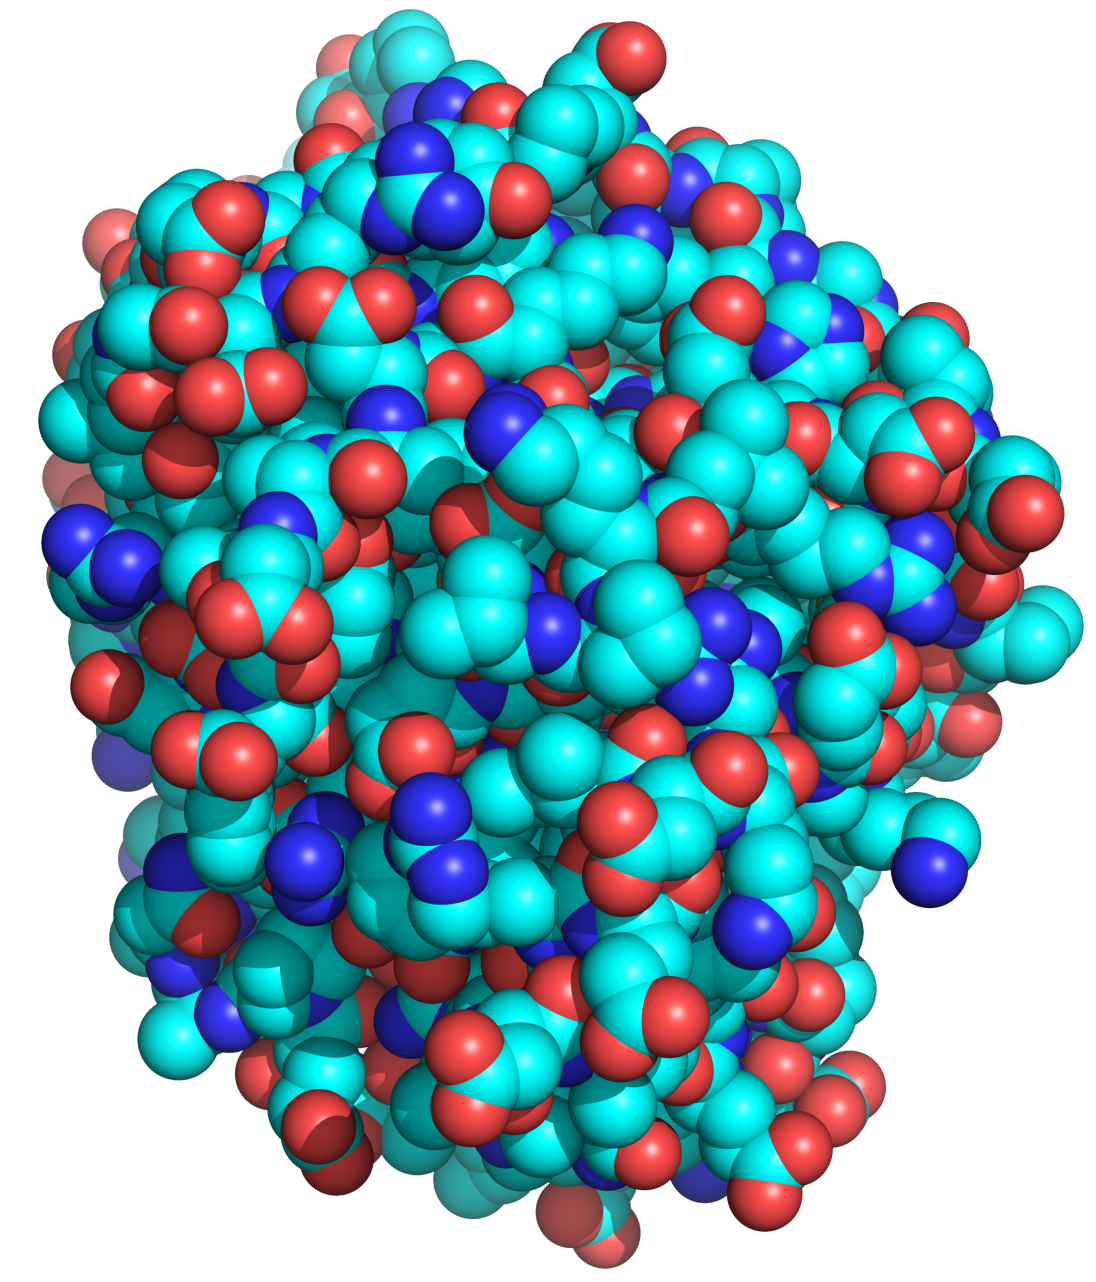
\includegraphics[width=0.15\textwidth]{fig/motiv1} &
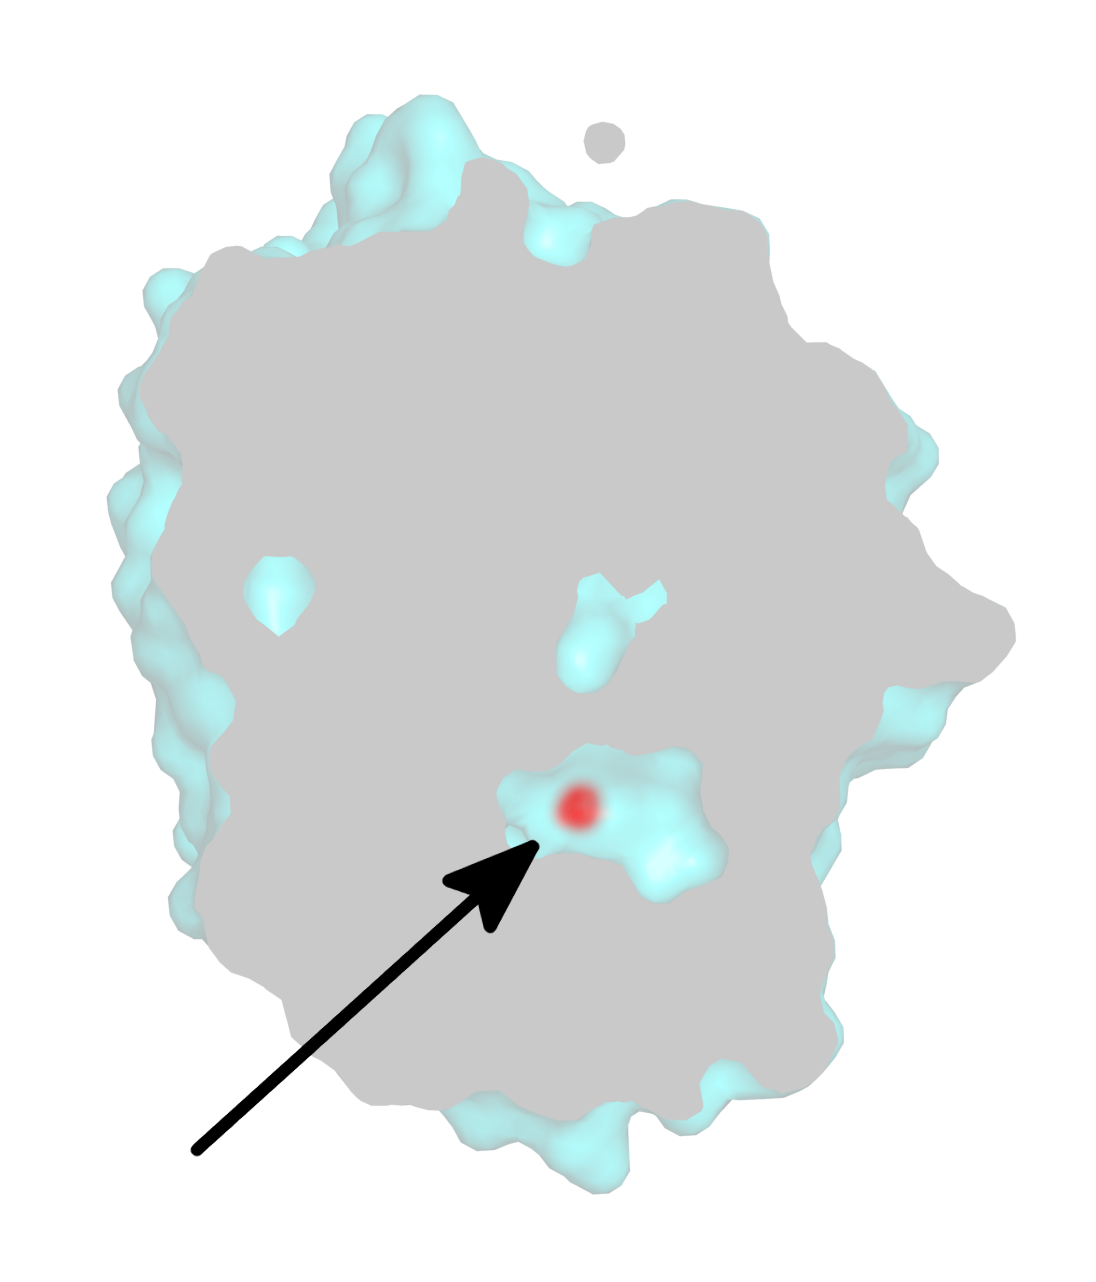
\includegraphics[width=0.17\textwidth]{fig/motiv2lab} &
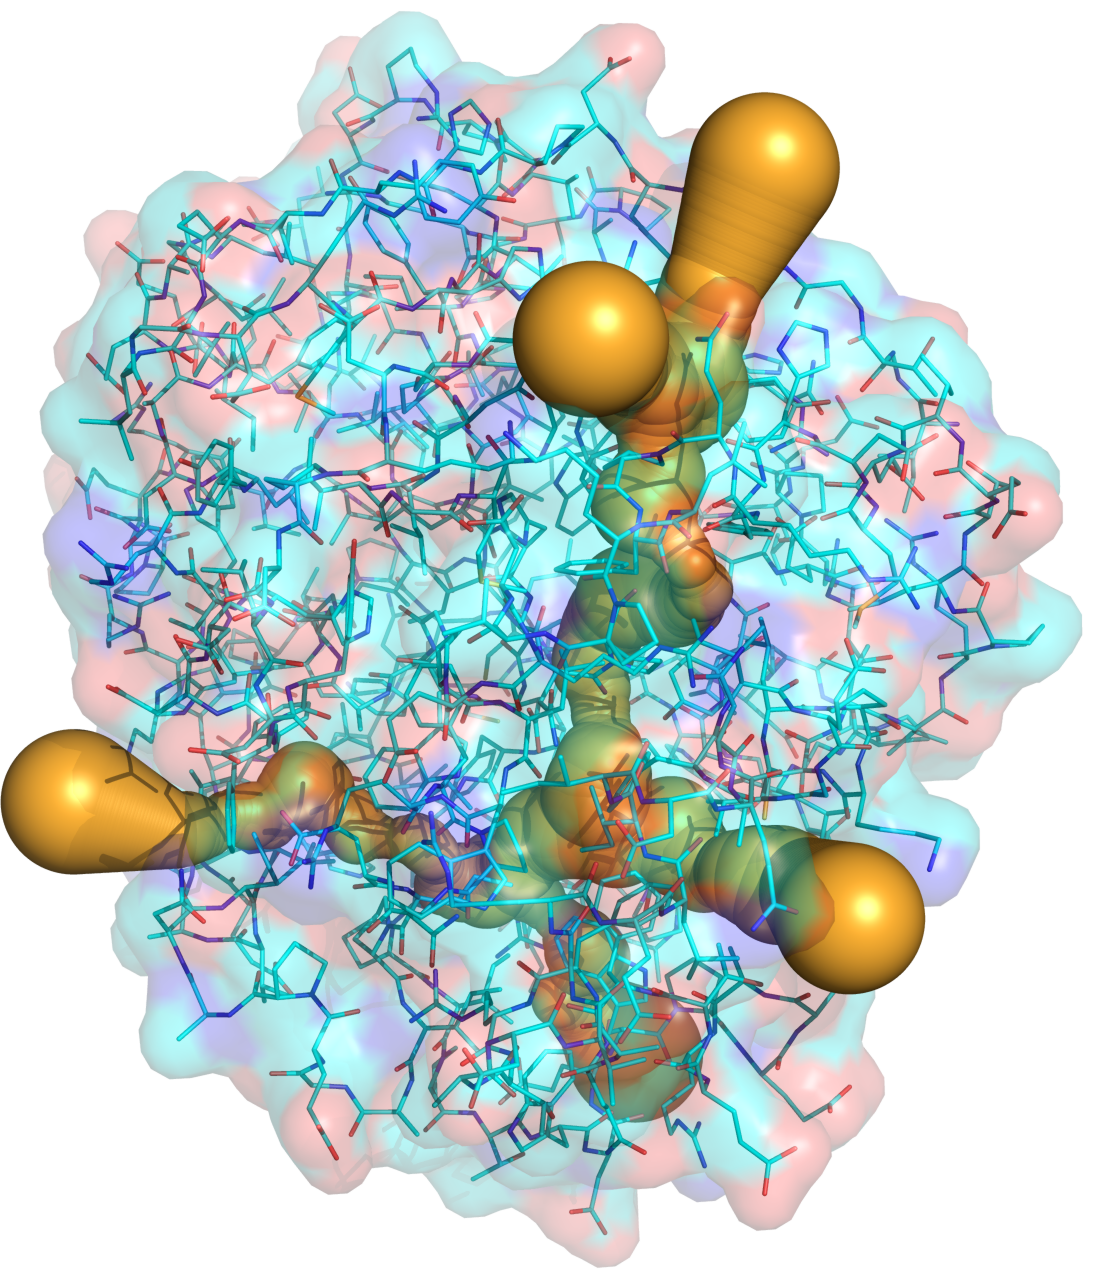
\includegraphics[width=0.16\textwidth]{fig/motiv3} &
\hbox{
\vbox{
\hbox{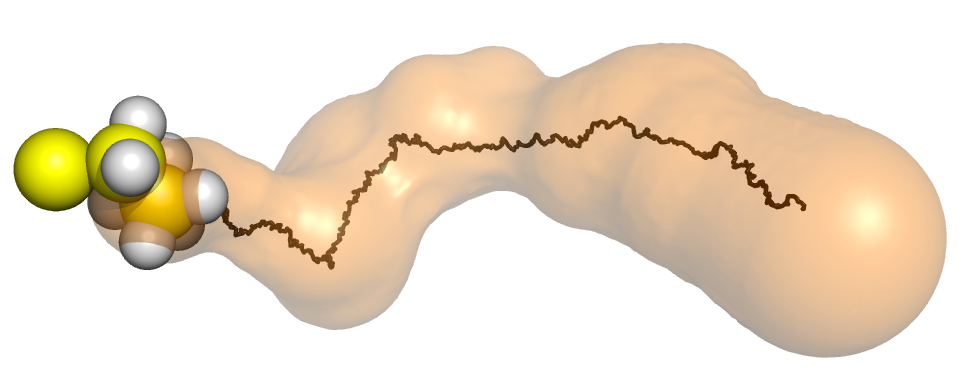
\includegraphics[width=0.25\textwidth]{fig/ta-1} }
\hbox{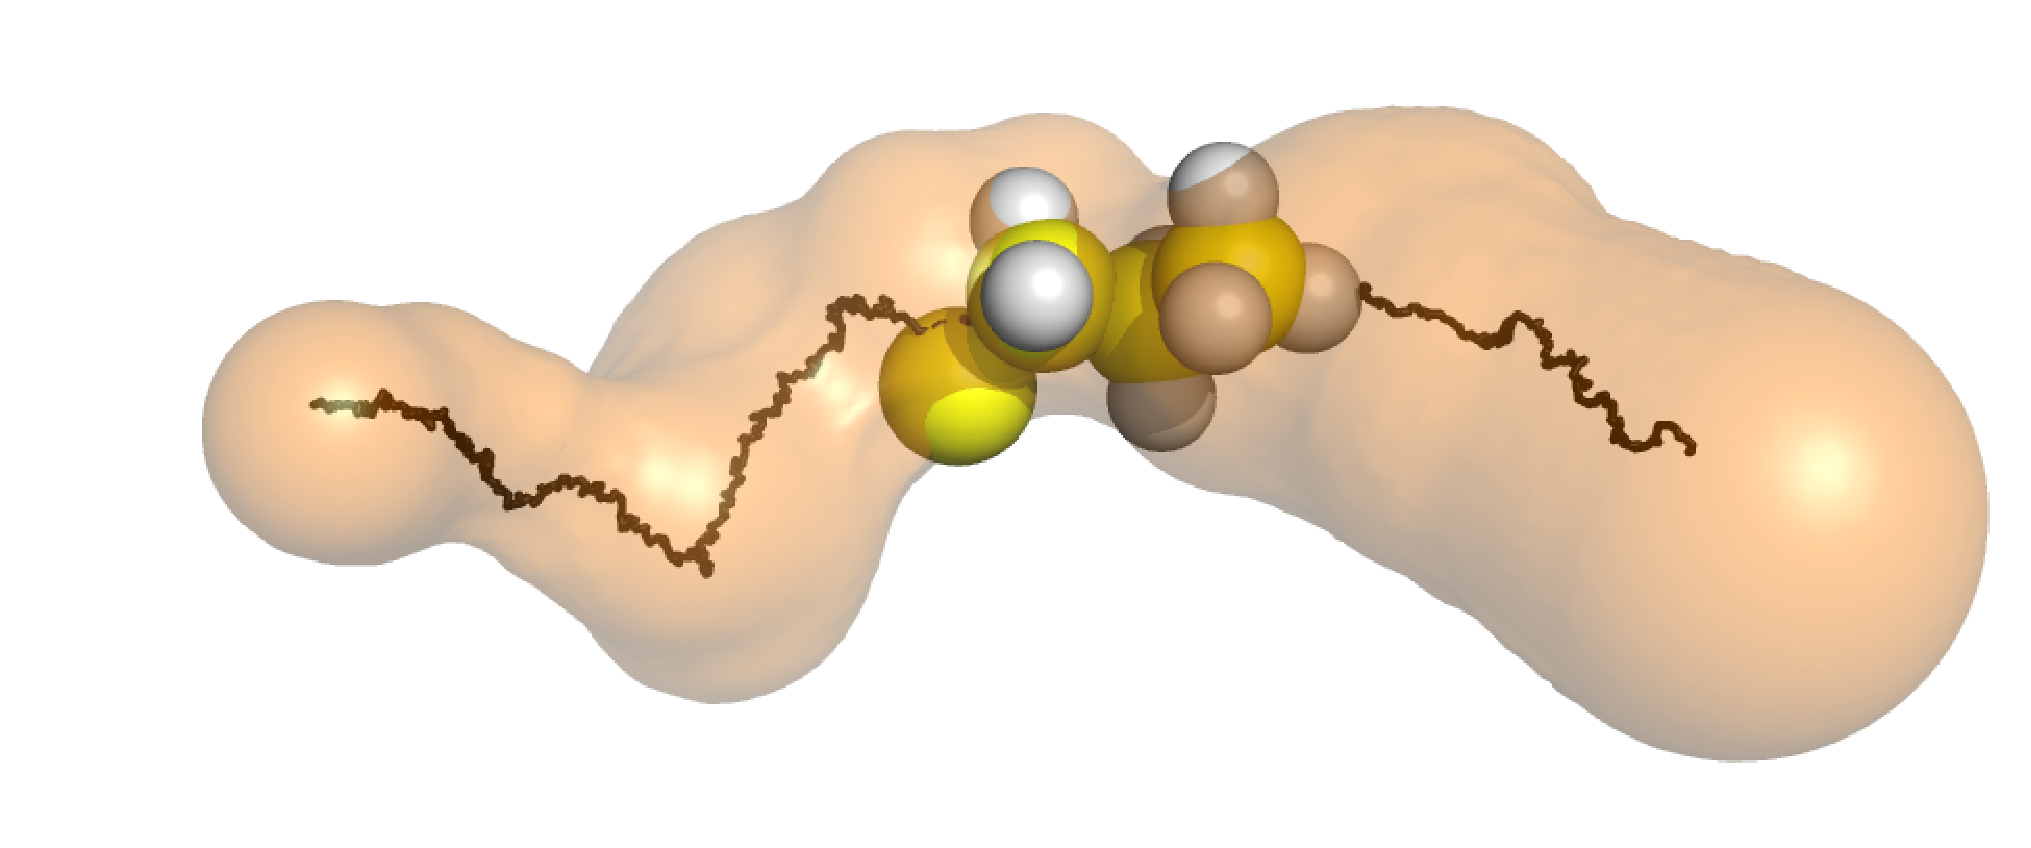
\includegraphics[width=0.25\textwidth]{fig/ta-433}}
} 
}
\\
Protein 1CQW & Active site & Detected tunnels & Example of a  \\
             &            & (orange)          & trajectory
\end{tabular}
}
\caption{\label{fig::motiv}
    Tunnels in haloalkane dehalogenase with a possible trajectory of 1-chlorpropan ligand.
}
\end{figure}

Understanding of interactions between proteins and other small molecules is crucial in many research fields, including drug design and protein engineering. 
These interactions are highly influenced by the ability to transport the small molecule, called ligand, to the protein active site.
The active site can be considered as a deeply buried inner cavity with the ability to interact with the incoming ligand.
To get the ligand to the active site, there has to be a transportation path connecting the protein outer environment with the active site.
These paths, called tunnels, have to be wide enough and the physico-chemical properties of the surrounding amino acids have to be compatible with the ligand (Fig.~\ref{fig::motiv}).

Traditionally, tunnels are detected using Voronoi diagrams~\cite{yaffe2008,caver3} assuming
%The widely used tools for tunnel detection are based on Voronoi diagrams~\cite{yaffe2008,caver3}.  %or a 3D grid~\cite{sehnal2013mole,petrek2006caver}.
 a spherical ligand (probe) and they are represented as a sequence of spheres.
Biochemists decide if a tunnel can be used to transport a given ligand mainly based on the tunnel length and bottleneck (i.e., the radius of the smallest sphere that forms the tunnel).
This is used for example in protein engineering, where the task is to change selected properties of a protein, e.g., its stability under different outer conditions~\cite{Koudelakova2013} or its activity of the protein towards other molecules~\cite{Pavlova2009}.
%The design of suitable ligands causing the desired changes can be speeded up by detecting and analyzing the tunnels leading to the active sites.
%This can be achieved by detecting and studying so called tunnels in proteins which can serve as the transportation paths for the 
%ligand from the outside environment to the active site or vice versa. 

Whereas the tunnel computation is already a well established research field, the simulation of ligand transportation through the detected tunnels is rather new.
Ligands are typically of non-spherical shape,therefore it is difficult to estimate their traversability through tunnels computed for a spherical probe.
The decision based only on spherical tunnels requires previous expertise in the domain and yet it may be imprecise.
To provide biochemists with a better insight into the behavior of non-spherical ligands, it is necessary to compute the trajectories of the ligand considering its shape and possibly also its conformation changes.

In this paper, we propose a novel method for computing the trajectories of flexible ligands in a tunnel.
The proposed work is based on the sampling-based Rapidly Exploring Random Tree (RRT)~\cite{lavalleRRT} planner.
The main idea of the proposed planner is to generate the random samples around a virtual sphere moving through the tunnel, which
guides the search in the configuration space.
This allows us to focus the sampling of the configuration space around the tunnel.
The flexibility of the ligand is modeled using a predefined set of typical conformations.
To enable ligand movements in narrow tunnels, a scaled-down version of the ligand is used, similarly, e.g., to~\cite{cortes2005path}.
It helps to keep also potential solutions which do not fit to the geometric restrains but can be still feasible because of the physico-chemical properties.
%This strategy helps to overcome the limitations of the conformational discretation introduced by the rotamer approximation.

The proposed method can be seen as an extension for the traditionally used tunnel detection tools.
%Besides trajectory computation, visualization of the results in important. %we also propose methods for their visualization.
Our motivation is to help the biochemists to perform so called virtual screening, where they test the traversability of a ligand through a given tunnel.
Therefore, methods for visualization of the results  are discussed.
In order to predict the success of ligand traversability, the virtual screening performs hundreds of thousands of tests and checks if the ligand passed through the tunnel.
The advantage of the proposed approach is that we can search the ligand path inside a specific tunnel which substantially decreases the computational time and resources required for the virtual screening.
%We further propose visualization techniques for presenting the results to biochemists.


\section{Related Work}


The analysis of protein structure aiming to reveal the tunnels has been supported by different computational software tools which take the geometry of the protein as an input and explore the inner void space (e.g., CAVER 1.0~\cite{petrek2006caver} or MOLE~\cite{Petrek20071357}). 
Early methods for tunnel detection utilized a discretized 3D grid, where each cell is considered as occupied or free depending
on the presence of atoms of the protein.
Tunnels can be then searched using standard graph-search methods, like Dijkstra's algorithm.
Besides, the grid can be used to identify other relevant properties like 
pockets, cavities, or channels~\cite{sehnal2013mole,petrek2006caver}.
%One of the first grid-based approaches to the detection of tunnels in protein is the CAVER 1.0 algorithm by Pet\v{r}ek et al.~\cite{citeulike:6257975}.
The obvious disadvantage of the grid-based methods is the high memory demand and their dependency on the grid resolution.
%Due to the high memory consumption, these methods are not suitable for tunnel detection in dynamic proteins and therefore they
%are used primarily for analysis of static molecules or individual snapshots of molecular dynamics.

Currently the most widely used approach to tunnel detection is based on ordinary Voronoi diagrams (VD) or Weighted Voronoi Diagrams (WVD).
The ordinary VD is computed on points representing centers of all atoms, without considering the radii of atoms.
%This may lead to detection of tunnels with incorrect bottlenecks. % i.e., incorrect radius of a smallest probe that can traverse the tunnels.
To consider atoms with different radii, the weights of individual points are determined by the van der Walls radii of atoms in WVD.
An alternative solution is to compute a non-weighted VD on an extended point set, where 
each atom is approximated by several spheres with a small radius~\cite{yaffe2008,caver3}.
VD-based methods are memory less demanding and also faster than the grid-based methods.
%The extension of VD-based methods to dynamic molecules requires to construct VD in the frames being analyzed and 
%finding correspondences between them.
%The existing approaches often use hierarchical clustering to match Voronoi vertices and edges from different frames, which is computationally demanding~\cite{lindow2012dynamic,caverDetails}.

The tunnels detected by the above mentioned approaches are evaluated using basic characteristics like bottleneck, length, curvature, and a list of surrounding
residues, which are later used to estimate the interaction possibilities.
The biggest disadvantage of both grid-based and VD-based methods is that the shape of the ligand is not taken into account during the tunnel detection and it is therefore not easy to estimate if (and how) a ligand might traverse the tunnels.
%The protein tunnels computed for spherical probes contain valuable information about the protein void space.
%Based on the biochemical properties, the chemists can decide if a given tunnel is relevant and can be possibly used by a ligand to exit the protein.
%The biochemically relevant tunnels can be then analyzed separately.

In order to determine if a ligand can pass the tunnel, it is necessary to compute a trajectory considering the shape of the ligand.
This can be formulated as a motion planning problem in a high-dimensional configuration space.
The configuration space $\C$ is formed by all possible configurations of the ligand in the tunnel, i.e., considering its rotation, translation, and possibly also other degrees of freedom responsible for the conformation changes.
The dimension of the configuration space is given by the degrees of freedom (DOF) of the ligand, i.e., 6D for a rigid ligand and 6D + $n$ for a flexible
ligand with $n$ DOFs.
Sampling-based motion planning methods can be used to search this high-dimensional configuration space~\cite{Lav06}.
The idea of sampling-based motion planning is to randomly sample $\C$ and classify the samples as free or non-free using collision detection.
The free samples are stored in a roadmap (a graph structure), in which a path can be searched using standard graph-search methods.

Sampling-based motion planning methods are suitable for computing the trajectories of the ligand as they 
can cope with many-DOF robots (objects) of arbitrary shapes.
The flexibility of ligands (or even proteins) can be modeled using a multi-link kinematic chain, where torsional angles
can change~\cite{songPFpath}.
This is useful, e.g., in the protein folding studies~\cite{al2012motion,gipson2012computational,amato2002using,raveh2009rapid} or analysis of loop motions~\cite{cortes2004geometric}.
%This is useful, e.g., in the protein folding studies~\cite{al2012motion,gipson2012computational,amato2002using,raveh2009rapid,novinskaya2015improving,songPFintro} or analysis of loop motions~\cite{cortes2004geometric}.
%Sampling-based methods have also been used for 
% tunnel detection~\cite{vonasek2016application,vonasek2017tunnel} and
% exit pathway computation~\cite{cortes2010simulating,guieysse2008structure}.
%none of the existing work focuses on the trajectory generation in tunnels.
%However, not all conformations are feasible, which has to be checked using potential energy, which is time consuming.

Rapidly Exploring Random Tree (RRT)~\cite{lavalleRRT} is a single-query sampling-based motion planning method that 
incrementally builds a configuration tree $\T$ rooted at the initial configuration $\qinit$.
In each iteration of RRT, a random configuration $\qrand \in \C$ is generated and its nearest node $\qnear \in \T$ in the tree is found.
A new configuration $\qnew$ is constructed on the line connecting $\qnear$ and $\qrand$ in the distance $\varepsilon$ from $\qnear$.
If $\qnew$ is collision-free, it is added to the tree.
The algorithm terminates if the tree approaches the goal configuration close enough.
%RRT is a suitable candidate for computing the trajectories of flexible ligands due to its ability to cope with many-DOF systems.

%rrt for molecular: \cite{al2012motion}
%survey \cite{gipson2012computational}
%In our previous works, we proposed to employ RRT also for the purp
%Solutions for tunnel detection using sampling-based methods however have not been discussed yet.
%Sampling-based planners have been used in various applications in robotics~\cite{elbanhawi2014sampling} and also  %,latombe1999motion} and also
% to study proteins, e.g. in  
%loop motions~\cite{cortes2004geometric},
%protein folding~\cite{amato2002using,raveh2009rapid,novinskaya2015improving,songPFintro},
%protein folding~\cite{raveh2009rapid,novinskaya2015improving},
%or protein folding combined with ligand diffusion~\cite{cortes2010simulating}.


%Two main issues need to be addressed: the increased dimension of the configuration space and the narrow passage problem.
%A well known issue of sampling-based planners is the narrow passage problem~\cite{hannaWIS}.

Motion planning for flexible ligands in protein tunnels brings two main issues: 
the ligand flexibility increases the dimension of the configuration space, and the necessity to plan in protein tunnels
leads to the narrow passage problem.
A narrow passage is a region in the configuration space whose removal changes the connectivity of the free space~\cite{hannaWIS}.
Narrow passages have smaller volume than other regions and it is therefore difficult to sample them dense enough using uniform distribution, that is used in the basic sampling-based planners.
The presence of narrow passages in the configuration space, especially if they contain part of the solution, requires many iterations
in order to put enough samples there and it consequently increases the planning time.
Typical tunnels have bottlenecks smaller than $1.0$~\AA, so they can already be considered as narrow passages for ligands with more than two atoms.
%The protein tunnels have the properties of the narrow passages, as they are very narrow
To cope with the narrow passages, they have to be sampled more dense.
For the family of RRT planners, it is useful to change the distribution of random samples according to the growth of the tree~\cite{vonasek2009rrt,vonasekphd,denny2016dynamic}.
%about their 3D position, which is represented by the tunnel centerline.
%The centerline can be used to guide the growth of the RRT tree through the configuration space~\cite{vonasek2009rrt,denny2016dynamic}.

%The additional degrees of freedom required to model the flexibility increase the dimension of the configuration space.
The kinematic chain representation used to model the ligand flexibility can generate all possible conformations but it also increases the dimension of the configuration space.
Not all of conformations are however feasible and it is therefore necessary to verify the feasibility of a given conformation based on energy, which is time consuming.
%RRT-based planners are sensitive to the employed metric, that should consider also the flexibility-related DOFs.
An alternative solution is to employ a library of known conformations.
The conformation changes of protein amino acids and ligand are represented by so called rotamers, stored in different rotamer libraries (e.g., Dunbrack library~\cite{dunbrack}).
Rotamers differ in the angles between their atoms.
Possible rotamer conformations correspond to energetically and geometrically favorable positions.
Using a library of predefined conformations is used also in other tasks, e.g.~\cite{kellogg}.
%This solution is common also in different types of calculations, e.g.~\cite{kellogg}. 


A RRT-based method for computing exit pathways for a small flexible molecule was presented in~\cite{cortes2010simulating}.
To cope with many-DOF ligands, the RRT-ML variant~\cite{cortes2007mlrrt} was employed.
RRT-ML expands the tree primarily using those DOF that are essential for achieving motion of the ligand (i.e., rotation
and translation) and it employs the other DOFs (i.e., that are responsible for conformation changes) if they hinder the growth of the tree.
The approach~\cite{cortes2010simulating} may however suffer from the narrow passage problem, as it aims to find some exit pathway for a given ligand, which requires to search the whole configuration space of the ligand/protein complex.
Although there are usually multiple pathways from a given active site, not all of them are traversable by a given ligand.
Many iterations are needed to find a solution, which increases the computational time.

In this paper, we propose to analyze the traversability separately for each tunnel.
This can bring several advantages for the biochemists.
The tunnels in a protein being studied can be computed using standard tunnel detection tools for spherical probes and assessed
according to their length, curvature, bottleneck, and biochemical properties (e.g., partial charge).
These characteristics are already used in many research studies.
Selected promising tunnels can be further analyzed for a given ligand to determine the traversability.
It is not necessary to first run time consuming MD simulations with both protein and ligand being studied, but it is suitable
to detected tunnels in the protein only.

The proposed work employs the RRT planning principle with three extensions: 
a) the configuration space is not sampled uniformly, but uses a guided sampling along the tunnel centerline,
b) the radii of the ligand atoms can be decreased, and 
c) ligand flexibility is modeled using a library of predefined conformations.
The first two extensions can help to deal with the narrow passage problem.
By reducing the scale of the atomic radii, the configuration tree can explore more areas of the configuration space.
The scaling-down technique have been used e.g. for motion planning of deformable objects~\cite{gayle2005path,alterovitz2008motion}, and
they are also used in the most related MoMa-LigPath tool~\cite{cortes2005path}.
%is used also in other related tools like like MoMa-LigPath~\cite{cortes2005path}
%Such techniques have been used for motion planning of deformable objects, 
%e.g., in~\cite{frank2008efficient,bayazit2001ligand,alterovitz2008motion,lamiraux2001flexible,kavraki1998towards,gayle2005path}, 
%e.g., in~\cite{frank2008efficient,bayazit2001ligand,alterovitz2008motion,lamiraux2001flexible,gayle2005path}, 
%and for motion planning of rigid objects among 
%flexible obstacles~\cite{rodriguez2006planning,frank2008efficient,phillips2014representation}.

%and the third modification
%is introduced in order to decrease the dimension of the configuration space.

%Ligands are small molecules interacting with the protein. 
%Due to the interaction, the relative positions of the ligand's atoms can change.
% in cortes2005path:
%In this paper two kinds of large-amplitude motion are treated: protein loop conformational changes (involving pro-
%tein backbone flexibility) and ligand trajectories to deep active sites in proteins (involving ligand and protein side-chain flex-
%ibility). First studies performed using our two-stage approach (geometric search followed by energy refinements) show that,
%    compared to classical molecular modeling methods, quite   similar results can be obtained with a performance gain of
% several orders of magnitude. Furthermore, our results also  indicate that the geometric stage can provide highly valuable information to biologists.
%This technique is similar to generation of samples near the medial exist of the environment
%medial axis~\cite{wilmarthMAPRM,foskey01hybrid,guibas1999probabilistic,hoff2000interactive,yang2004adapting,amatoOBRRT}.
%or by guiding the growth of the tree around a general path in the workspace~\cite{vonasek2009rrt,denny2014marrt}.

\section{Traversability of Tunnels}

\subsection{Preliminaries}

Proteins and ligands are represented by the hard sphere model, where the radius of each sphere (atom) is given by its van der Waals radius.
The flexibility of a ligand is modeled using the set $\L$ of its conformations.
The conformations $L$ are used from a library (e.g.,~\cite{dunbrack}), or they can be prepared considering the potential energy.

%or downloaded from a library~\cite{dunbrack}.
%We assume that a conformation $l \in \L$ can be switched to all other conformations in $\L$.

%Another approach is to model the ligand flexibility using a predefined set of feasible conformations $\L$
%To decrease the computational burden, a set of feasible conformations $\L$ is prepared, e.g. using Rosseta tool.
%The conformations can be prepared using Molecular Dynamics software such as Rosetta.
%For each conformation $c\in \L$ an energy potential is also calculated.
%Let $\L_i$ denote the set of conformations that 
%The transition matrix $M$ defines the possible changes of conformations, i.e., $M(i,j)=1$ if the conformation $c_i \in C$
%can be switched to the confomration $c_j \in C$.

A protein tunnel is described by a sequence of collision-free spheres 
$T=( (c_1, r_1),\ldots,(c_n,r_n) )$, where $n$ denotes the number of spheres,
$c_i \in \R^3$ is their 3D position and $r_i > 0$ denotes the maximum collision-free radius of a sphere centered at $c_i$. 
The tunnels can be found by tunnel detection tools like CAVER 3.0~\cite{caver3}.

%from wiki:
%Multiple static structures experimentally determined for the same protein in different conformations are often used to emulate receptor flexibility.[19] Alternatively rotamer libraries of amino acid side chains that surround the binding cavity may be searched to generate alternate but energetically reasonable protein conformations.[20][21]
% 19 = \cite{totrov2008flexible}
% 20 = \cite{hartmann2009docking}
% 21 = \cite{taylor2003fds} 

%Conformations of the ligand may be generated in the absence of the receptor and subsequently docked[13] 
%or conformations may be generated on-the-fly in the presence of the receptor binding cavity,[14] 
%or with full rotational flexibility of every dihedral angle using fragment based docking.[15] 
%Force field energy evaluation are most often used to select energetically reasonable conformations,[16] but 
%knowledge-based methods have also been used.[17]
%13 = https://link.springer.com/article/10.1007/BF00123666

%The proteins are dense structures and the tunnels are typically narrow.
%Depending on the protein, the tunnel bottlenecks can be even less than $1$~\AA, which is too narrow for ligands with more than 2 atoms.
To enable motion of ligands in the narrow tunnels, the atomic radii of the ligand are scaled down by a factor $s, 0 < s \le 1$.
A discrete set of scales is used, i.e., $s \in \{\smin, \smin+\sdelta, \ldots, \smax\}$, where 
$\smin$ is the minimal allowed scale, $\smax=1$ is the maximal allowed scale and $\sdelta$ is the minimal difference between two scales.

A configuration of the pseudoflexible ligand $q=(x,y,z,r_x,r_y,r_z,l,s)$  is described
by the 3D position $(x,y,z)$ of the reference point of the ligand (e.g., its geometric center), rotation around $x$, $y$, and $z$ axes,
index of the conformation $l\in \L$ and the actual scale $s$.
All possible configurations form the configuration space $\C$. 
A configuration is collision-free if none of the ligand atoms scaled by $s$ and placed at the
position defined by $q$ collides with the protein atoms.
%The set of all feasible configurations at scale $s$ is denoted $\CFD \subseteq \C$.


\subsection{Computing Initial Configuration}

The analysis of tunnel traversability is based on computation of multiple trajectories of the ligand inside the tunnel, which
requires to generate a set $\QI$ of collision-free initial configurations.
In this paper we assume that the ligand has to travel from the beginning to the end of the tunnel.
As the tunnel are computed for a spherical probe, the ligand may not fit exactly to the first sphere of the tunnel.
The initial configurations have to be searched around the first sphere of the tunnel.
To find a new initial configuration, a random sample $q$ is generated around $c_i$ in the distance $\RI$ (translation and rotation
 parts of $q$ are generated randomly, the scale is set to $\smin$ and the conformation index is set randomly).
If the sample $q$ is collision-free, it can be considered as a new starting configuration, so $q$ is added to $\QI$.
Similarly, a single goal configuration $\qgoal$ is found around the end of the tunnel. 
For each starting configuration $\qinit \in \QI$,  $K$ trajectories are created.
Each trajectory is computed using a modified RRT, which is introduced in the following section.


\subsection{Computing Single Trajectory of the Ligand}

The task of the trajectory computation is to find a trajectory for the given ligand in the given tunnel. 
% which can be solved using RRT~\cite{lavalleRRT}.
Here, the original RRT is extended to cope with the specific requirements needed for the traversability of ligands.
First, the trajectory has to be found around the given tunnel, but deflection from the tunnel centerline is allowed.
%The deviation of the trajectory from the tunnel centerline is influenced by the parameter $\rv$.
%We assume, that the distance of the ligand from the tunnel centerline is at most $\rv$.
Due to this requirement, sampling process of RRT has to be adapted in order to follow the tunnel, and to prevent
construction of trajectories in the rest of the protein.
%The other modifications aim to cope with various scales of the ligand and multiple conformations,

The main loop of the proposed method is described in Alg.~\ref{alg::main}.
In each iteration, a random sample $\qrand$ is generated and its nearest node $\qnear\in\T$ in the tree is found.
The nearest-neighbor search between the $\qrand$ and the tree is performed using the weighted 6D Euclidean metric considering
both 3D rotation and 3D translation.

To guide the growth of the tree through the tunnel, a moving virtual goal is used~\cite{vonasek2009rrt}.
The virtual goal $v, 1\le v \le n$, is the index of sphere of the tunnel.
The random samples $\qrand$ are generated with probability $1-\gb$ from $\C$, otherwise they are generated around the sphere $c_v \in T$.
After the tree reaches the sphere $c_v$, i.e., the distance of the tree to $c_v$ is
less than a predefined threshold $\dt$, the virtual goal is moved to the successor of the last sphere in the tunnel
that is reached by the tree (lines~\ref{alg::main:a}--\ref{alg::main:b} in Alg.~\ref{alg::main}).
Setting the virtual goal to this successor allows the tree to avoid such parts of the tunnels that are not traversable or reachable by the ligand.
This is necessary in the dense protein structures, where it is not always possible to exactly follow the tunnel.
The algorithm terminates after a predefined number of planning trials $\Imax$ or if the tree reaches
the last sphere in the tunnel, i.e., when $v = n$.

To generate the samples $\qrand$ around the virtual goal $v$, the translation part $(x,y,z)$ of $\qrand$ is generated
from $N(c_v,\Sigma)$, where $\Sigma$ is the diagonal matrix with diagonal entries equal to the parameter $\rv$, and the rotational
part of $\qrand$ is generated using techniques described in~\cite{kuffnerES}.
The other two parameters (ligand index $l$ and scale $s$) of $\qrand$ can be left zero, as these are not used in the employed
metric for the nearest-neighbor search.
The parameter $\rv$ influences the distribution of samples around the tunnel centerline. 
By setting $\rv$ to a small value, the planner attempts to find the trajectories inside the tunnel, while higher values
of $\rv$ cause  exploration of paths around the tunnel.
We propose to set this parameter to the average tunnel width.

\linesnumbered
\begin{algorithm}[h]
{\small
\setstretch{0.88}
\caption{\label{alg::main}Main loop of the RRT planner}
\KwIn{
    tunnel $T=( (c_i, r_i) )$, $i=1,\ldots,n$, with spheres centers $c_i \in \R^3$ and radii $r_i$,
    initial configuration $\qinit$
%    goal configuration $\qgoal$,
}
\KwData{
   ligand conformations $\L$,
   scale limits $\smin, \smax$ and $\sdelta$
}
\KwOut{
    configuration tree $\T$\;
}
\hrule
$v = 1$; // index of the virtual goal\\
$iteration = 0$\;
\While{$iteration < \Imax$ {\bf and}  $v < n$}{
    \eIf{$rand() < \gb$}{
        $\qrand$ = random sample around actual virtual goal $c_v \in T$\;
    }{
        $\qrand$ = random sample from $\C$\;
    }
    $\qnear$ = nearest node in $\T$ towards $\qrand$\;
    expand($\qnear,\qrand$)\;
    \For{$i= n-1,n-2,\ldots,v+1,v$}{ \nllabel{alg::main:a}
        $d$ = nearest node in the tree towards sphere $c_i$\;
        \If{$d < \dt $}{
            $v = i+1$; // new virtual goal found\;
            {\bf  break}\;
        }
    } \nllabel{alg::main:b}
    $iteration = iteration+1$\;
}
\return $\T$\;
}
\end{algorithm}


The core of the proposed planner is the expansion procedure (Alg.~\ref{alg::expand}) which generates new collision-free nodes around $\qnear\in\T$.
For each ligand conformation $l \in \L$, the expansion procedure attempts to find a new collision-free configuration around $\qnear$ with a maximal scale.
First, the maximal scale $\smax$ is tested and $m$ random samples are generated around $\qrand$ and tested for collision.
The nearest collision-free sample towards $\qrand$ is selected and added to the tree.
If none of the tested samples is collision-free, the scale is reduced to $\smax-\sdelta$ and the search continues
until a collision-free sample is found or until the minimal reduced-scale $\smin$ is reached.
The random samples are generated similarly as in the case of $\qrand$ samples, only their translation
part is generated around $\qnear$.

The sampling-based methods are sensitive to the employed metric, especially if the objects are not symmetrical, which is the
case of the non-spherical ligands.
To consider the actual shape of the ligand (which is different in each conformation) and to allow finding such configurations
that approach $\qrand$, the distance between newly generated configurations and $\qrand$ is measured as the smallest
3D distance between an atom of the ligand placed at $q$ and the 3D position of $\qrand$ ($\da(q,\qrand)$ on line~\ref{alg::expand:a} in
Alg.~\ref{alg::expand}).
By computing the distance between the nearest atoms, the shape of the ligand is actually considered.
As the expansion routine attempts to find such sample that minimizes this distance to $\qrand$, it supports retraction
of the ligand towards $\qrand$.


\begin{algorithm}[h]
{\small
\setstretch{0.88}
%\setstretch{\straa}
\caption{\label{alg::expand}expand}
\KwIn{
   configuration $\qnear$ to be expanded,
   random configuration $\qrand$
}
\KwData{
   ligand conformations $\L$,
   scale limits $\smin, \smax$, and $\sdelta$,
   tree $\T$
}
%\KwOut{
%    set $S$ of collision-free configurations reachable from $\qnear$\;
%}
\hrule
\ForEach{$l \in \L$}{
    \ForEach{$s \in (\smax,\smax-\sdelta, \ldots, \smin+\sdelta, \smin)$}{
        $\qnew = \emptyset$; // empty configuration\\
        \For{$i = 1,\ldots,m$}{
            $q=\qnear$\;
            $q.position$ = random 3D position around $\qnear$\;
            $q.rotation$ = random 3D rotation\;
            $q.l = l$\; 
            $q.s = s$\;
            \If{isCollisionFree($q$)}{
                \If{$\qnew = \emptyset$ {\bf or} $\da(q, \qrand) < \da(\qnew,\qrand)$}{ \nllabel{alg::expand:a}
                    $\qnew = q$\;
                }
            } 
        }
        \If{$\qnew \ne \emptyset$} {
            $\T$.addNode($\qnew$)\;
            $\T$.addEdge($\qnear,\qnew$)\;
            {\bf break;} // go to next conformation
        }
    }
}
}
\end{algorithm}

The result of each planning trial is the tree $\T$ of collision-free configurations in which a path
between $\qinit$ (root of the tree) and $q'$ is found, where
 $q'$ is the nearest node in the tree towards $\qgoal$ (using 3D Euclidean metric). 
The path $P=(q_i), q_i \in \C$ is represented as a sequence of collision-free configurations.
The path is found in the tree even if the tree does not approach $\qgoal$ close enough.
Considering also these non-feasible solutions is necessary to evaluate difficult areas of the tunnels, e.g. bottlenecks.
The utilization of all computed paths for evaluation of tunnel difficulty is described in the next section.


\subsection{Traversability Characteristics}

For each initial configuration $\qinit \in \QI$, $K$ trajectories are computed, which results in the set of $K |\QI|$ trajectories.
All these trajectories are used to compute the following properties of the tunnel $T$.
A trajectory $P$ reaches the tunnel sphere $c_i \in T$, if the 3D Euclidean distance of the 
nearest configuration $q \in P$ towards $c_i$ is less than $r_i$ (radius of the sphere $c_i$).
Let $N(i)$ denote the number of trajectories that reached $i-$th sphere of the tunnel, $i=1,\ldots,n$.
Three basic characteristics of the tunnel are computed from the trajectories: accessibility, throughput, and the scaling factor.

The accessibility $A(i)=N(i)/N$ of the sphere $i$ is the probability of reaching the sphere $i$, where $N=K|\QI|$ is the total number of trajectories.
The accessibility shows how probable it is to pass the tunnel up to the sphere $i$.
Obviously, the most important is $A(n)$ of the last sphere of the tunnel, which can be considered as the overall difficulty of the tunnel.
The  ligand passage may however be strongly affected by the first bottleneck, so the parts of the tunnel located behind
the bottleneck have low accessibility.

%To better measure the probability of passing a given tunnel part, we should take into account only trajectories that even have chance
%to visit this part, e.g., the trajectories that reached the preceding tunnel part.
The throughput $T(i)$ is the ratio of trajectories that passed sphere $i$ (i.e., visited sphere $i+1$) and reached the sphere $i$,
i.e., $T(i) = N(i+1) / N(i)$. 
The throughput is not computed for the last sphere ($i=N$).
The throughput shows a local accessibility of tunnel parts and it can be used to detect places where most of the trajectories ends.

%The probability of the ligand that it reaches a tunnel's part.
%We employ the tunnel representation from CAVER 3.0 and we define a tunnel part as a sphere $P = (x, r)$ where $x \in \mathbb{R}^3$ is sphere center and $r \in \R$ is its radius.
%Then, for each trajectory $t$ we define its ending tunnel part $P_t^e$ as the part whose center is closest to the end position of $t$.
%Finally, the accessibility of $P$ is defined as a ratio of trajectories that passed $P$ or ended in $P$ over all trajectories.
%On the other hand, the probability does not show any details about the ligand's passage, e.g., how complicated it is to pass through some part of the tunnel, which trajectory is the most used one, etc.
%Moreover, it is not feasible to directly visualize and explore the resulting trajectories due to the visual clutter (see Fig.~\ref{fig:trajectories} left) caused by their high number and close proximity.

The proposed planner is allowed to scale down the radii of ligand spheres up to the allowed scale $\smin$. 
It can be expected that narrower parts of the tunnel are more often passed with a more scaled-down ligand than
the wider parts.
Ligand scale $L(i)$ at the tunnel sphere $i$ is the average scale of ligand that reaches the sphere $i$.
%The ligand scale is computed as the average value of scales of the nearest configurations of the trajectories towards tunnel sphere~$i$.

%--- The scale of the ligand when it passes a given tunnel's part.
%For the trajectory $t$, the ligand scale $s(P_t)$ in the tunnel part $P_t$ is defined as the scale of such sample of $t$ whose position is the closest one to the center of $P_t$.
%Then, the average ligand scale is defined as $s(P) = \frac{1}{|T|} \sum_{t \in T} s(P_t)$.
%Similarly, the minimum and maximum ligand scales can be defined.


\subsection{Visualization of Results}

%In order to fursupport the tunnel exploration process performed by biochemists.
The above defined characteristics can be shown even as a graph, or better, presented visually by mapping them using colors to the tunnel spheres.
 Alternatively, the surface representation can be used to visualize the tunnel.
In this case, a 3D point on the tunnel surface is colored according to the property value in its nearest tunnel part $i$,  i.e., such part $i$ whose center $c_i$ is the closest to the point among all tunnel parts.

The examples of the color mapping are shown in Fig.~\ref{fig:properties}.
The accessibility (Fig.~\ref{fig:properties}a) shows that more than the half of the tunnel is not accessible (red part of the tunnel).
The throughput shows (Fig.~\ref{fig:properties}b) that the only difficult is the part around the bottleneck (red color in Fig.~\ref{fig:properties}b), and the second half of the tunnel is also traversible.

\begin{figure}[h]
\centering
\begin{tabular}{ccc}
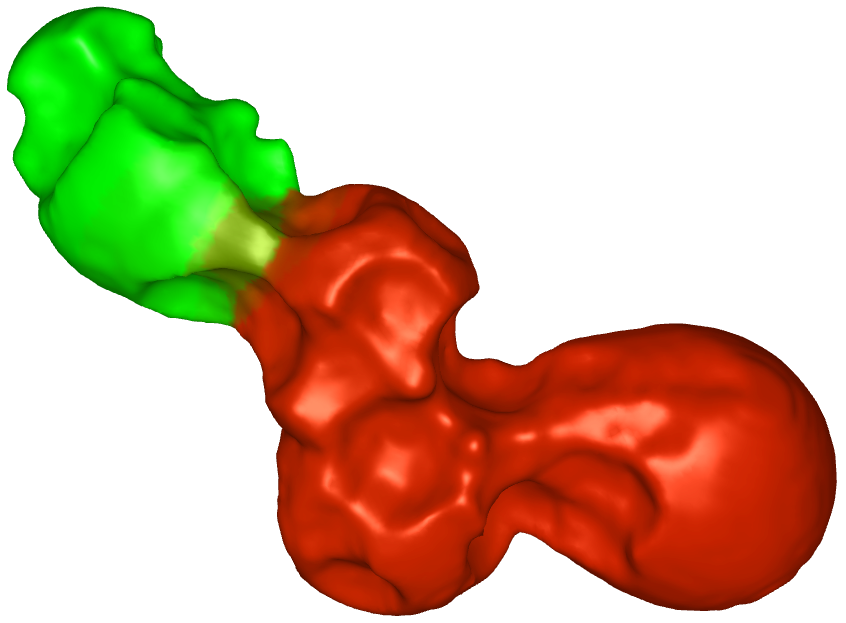
\includegraphics[width=0.3\textwidth]{fig/accessibility} &
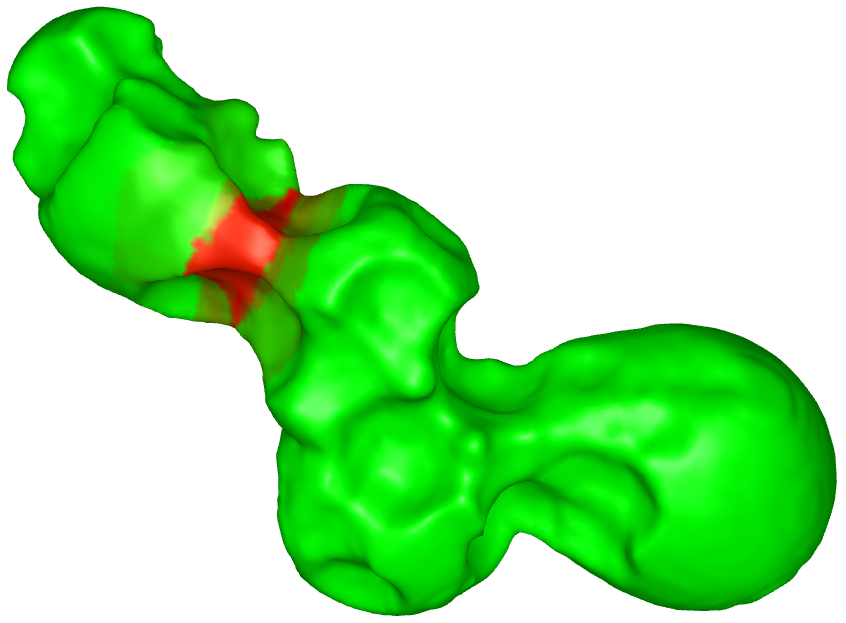
\includegraphics[width=0.3\textwidth]{fig/throughput} &
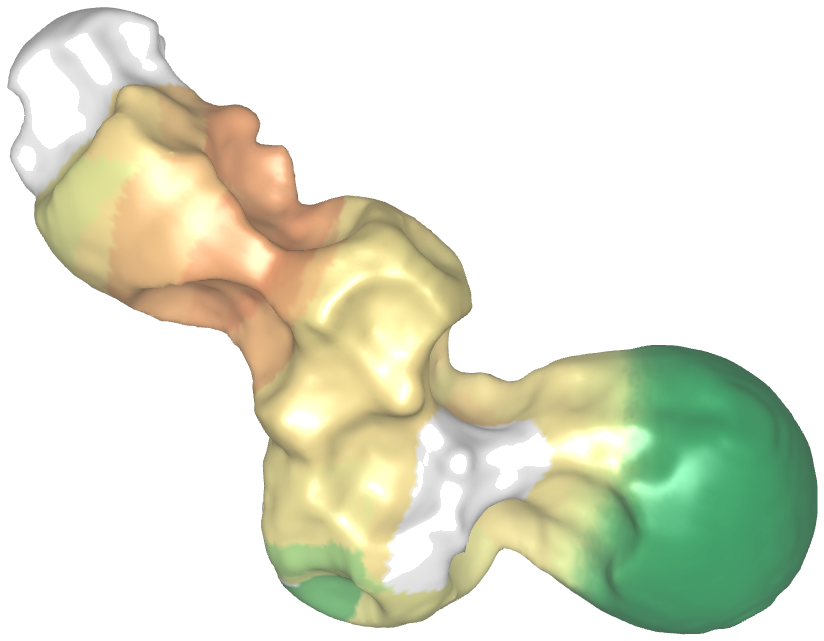
\includegraphics[width=0.3\textwidth]{fig/ligand-scale} \\
  (a) & (b) & (c) \\                     
\end{tabular}
\caption{Tunnel properties mapped onto its surface. The tunnel begins at the top left corner.
(a) Accessibility --- green denotes the parts that were accessed by the ligand easily ($A(i) > 80$~\%), 
    while red denotes parts that were accessible  in $<10$~\% of cases.
(b) Throughput --- green denotes parts that are highly probable to be passed by the ligand ($T(i) > 80$~\%), 
    while red denotes those that were hard to pass ($T(i) < 20$~\%).
(c) Ligand scale --- the average scale of the ligand was \tylde 50\% in orange parts, \tylde 60\% in yellow parts, \tylde 80\% in yellow to green parts and \tylde 100\% in green parts.
\label{fig:properties}
}
\end{figure}



\def\cstart{\overline{c_{start}}}
\def\cend{\overline{c_{end}}}

Besides the color mapping, it is also necessary to show the computed trajectories.
%This is useful, for example, to find out in which part of the tunnel the trajectories detour.
Simple visualization of all trajectories could however be too slow for an interactive work.
Therefore, the trajectories are first clustered and then only the clusters are visualized.
Due to different lengths of the trajectories, they are first converted to a normalized form.
Let $\cstart$ represent the average starting position of all trajectories and let $d_{max}$ be the 3D Euclidean distance
of the most distant configuration from $\cstart$ amongst all trajectories.
A set of $M$ spheres centered at $\cstart$ are created with radii $r'_i=i {d_{max} \over M}$, where $i=0,\ldots, M-1$.
The trajectory $P=(q_1,\ldots,q_n)$ of length $n$ is represented by the normalized vector $v=(x_1,\ldots,x_M)$ of length $M$,
where $x_i$ is the 3D position of the nearest configuration $q \in P$ to the surface of the $i$-th sphere with the radius $r'_i$.
The distance between two normalized trajectories $v_i$ and $v_j$ is defined as
$d(v_i, v_j) = \frac{1}{M} \sum_{1 \leq k \leq N} |x_k^i x_k^j|$.
This distance is used in the UPGMA clustering technique~\cite{sokal1958statistical}.
The trajectories can be visualized using a representative of each cluster.
The number of trajectories in each cluster is represented by the width of the polyline (Fig.~\ref{fig:trajectories}).
%In this manner, we are able to convey the information about all different trajectories together (see Fig.~\ref{fig:trajectories} right).

\begin{figure}
\centering
\begin{tabular}{cc}
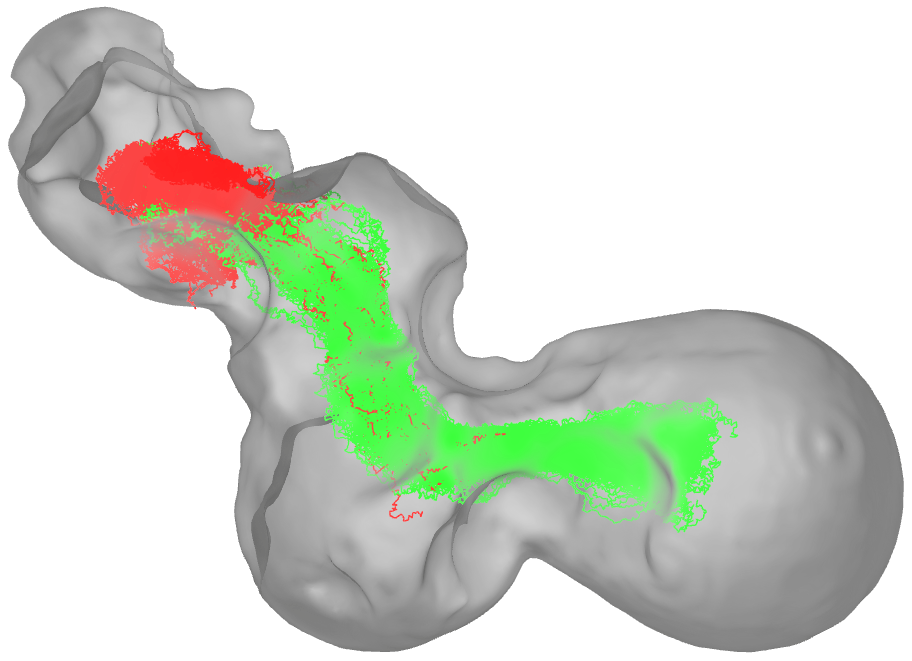
\includegraphics[width=0.4\textwidth]{fig/trajectories-all} &
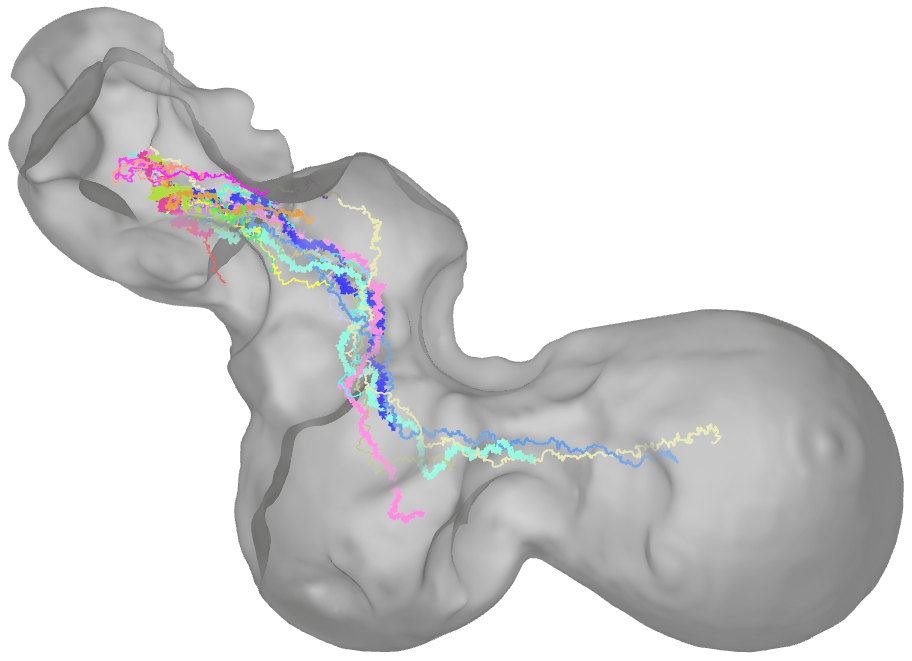
\includegraphics[width=0.4\textwidth]{fig/trajectories-clustered-21} \\
(a) & (b) \\                       
\end{tabular}
\caption{Visualization of the trajectories. The tunnel begins in the top left corner.
(a) All trajectories ($\sim5000$) colored according to whether they reached the end of the tunnel (green) or not (red). 
(b) Visualization using clusters of trajectories. 
%Trajectories clustered according to their proximity colored by distinct colors.
%The different line widths represent the number of trajectories in a cluster.
\label{fig:trajectories}
}
\end{figure}




\section{Experimental Verification}

The tunnels in Haloalkane dehalogenase protein (PDB ID 1CQW) has been analyzed using the proposed approach.
Three tunnels were detected using CAVER 3.0~\cite{caver3} for the spherical probe of radius 0.9~\AA (Fig.~\ref{fig::tunnel}a).
The traversability was evaluated for 1-chlorpropan (denoted as $\LA$) with 11 atoms and 
% from David: m003 je "1-chlorpropan" a m004 "1-chlorbutan"
and 1-chlorbutan (denoted as $\LB$) with 14 atoms.
$\LA$ was represented by 12 conformations, and $\LB$ by a set of $114$ conformations.
Examples of three conformations of $\LA$ and $\LB$ are depicted in Fig.~\ref{fig::tunnel}b.
Further information about the experiments can be found at {\url{http://mrs.felk.cvut.cz/isrr2017}}.

Both tested ligands have more than 10 atoms and therefore they cannot fit into the tunnel of with 0.9~\AA, so
the radii of ligands were scaled down. 
Four different scaling-down factors were used: $\smin=\{0.3,0.4,0.5,0.6\}$.
No trajectories were found for $\smin > 0.6$.
For each scale, 50 collision-free initial configurations were found in the $\RI=2$\AA\ radius around the first sphere of the tunnel.
For each ligand, each minimal scale $\smin$ and each initial configuration, 100 trajectories were computed using the proposed planner.
The parameters of the planner were: $\Imax=10,000$, $m=50$, $\gb=0.9$, $\dt=1.5$\AA, $\rv=2$~\AA.
For each initial configuration, the success rate is computed as the ratio of trajectories that reached the end of the tunnel (to the distance 
 $\rv=2$~\AA or less) over 100 trials.

The average runtimes, success rates and sizes of the built trees for the first tunnel are shown in Tab.~\ref{tab::rrt}.
The highest average success rate wasv achieved for the most scaled-down ligands ($\smin=0.3$) and it decreases with the increasing $\smin$. 
The difference between the minimal and maximal success rates indicates how the initial configurations of the ligand influence the ability to pass the tunnels.
For example, the most difficult initial configuration of $\LA$ and $\smin=0.3$ lead to success rate 78~\% (the easiest 
        initial configuration lead to success rate $100$~\%), but for the scale $\smin=0.4$, the worst success rate is
only $42$~\% and the best 96~\%.
The traversability of larger ligands ($\smin=0.4$ vs. $\smin=0.3$) is therefore more sensitive to the initial configuration.
This shows the importance of testing the traversability from multiple initial configurations.
The runtime is significantly higher for the $\LB$ ligand, which is caused by the larger number of conformations that need to be
examined in each expansion.

%The tree can be expanded by up to $|\L|$ conformations in each iterations, which gives theoretical
%size of the tree $110\cdot 10^3$ for $\LA$ and $1140\cdot 10^3$ for $\LB$.
%The constructed tree are however significantly smaller


\def\tmpa{0.13\textwidth}

\begin{figure}
\centering
\begin{tabular}{cc}
%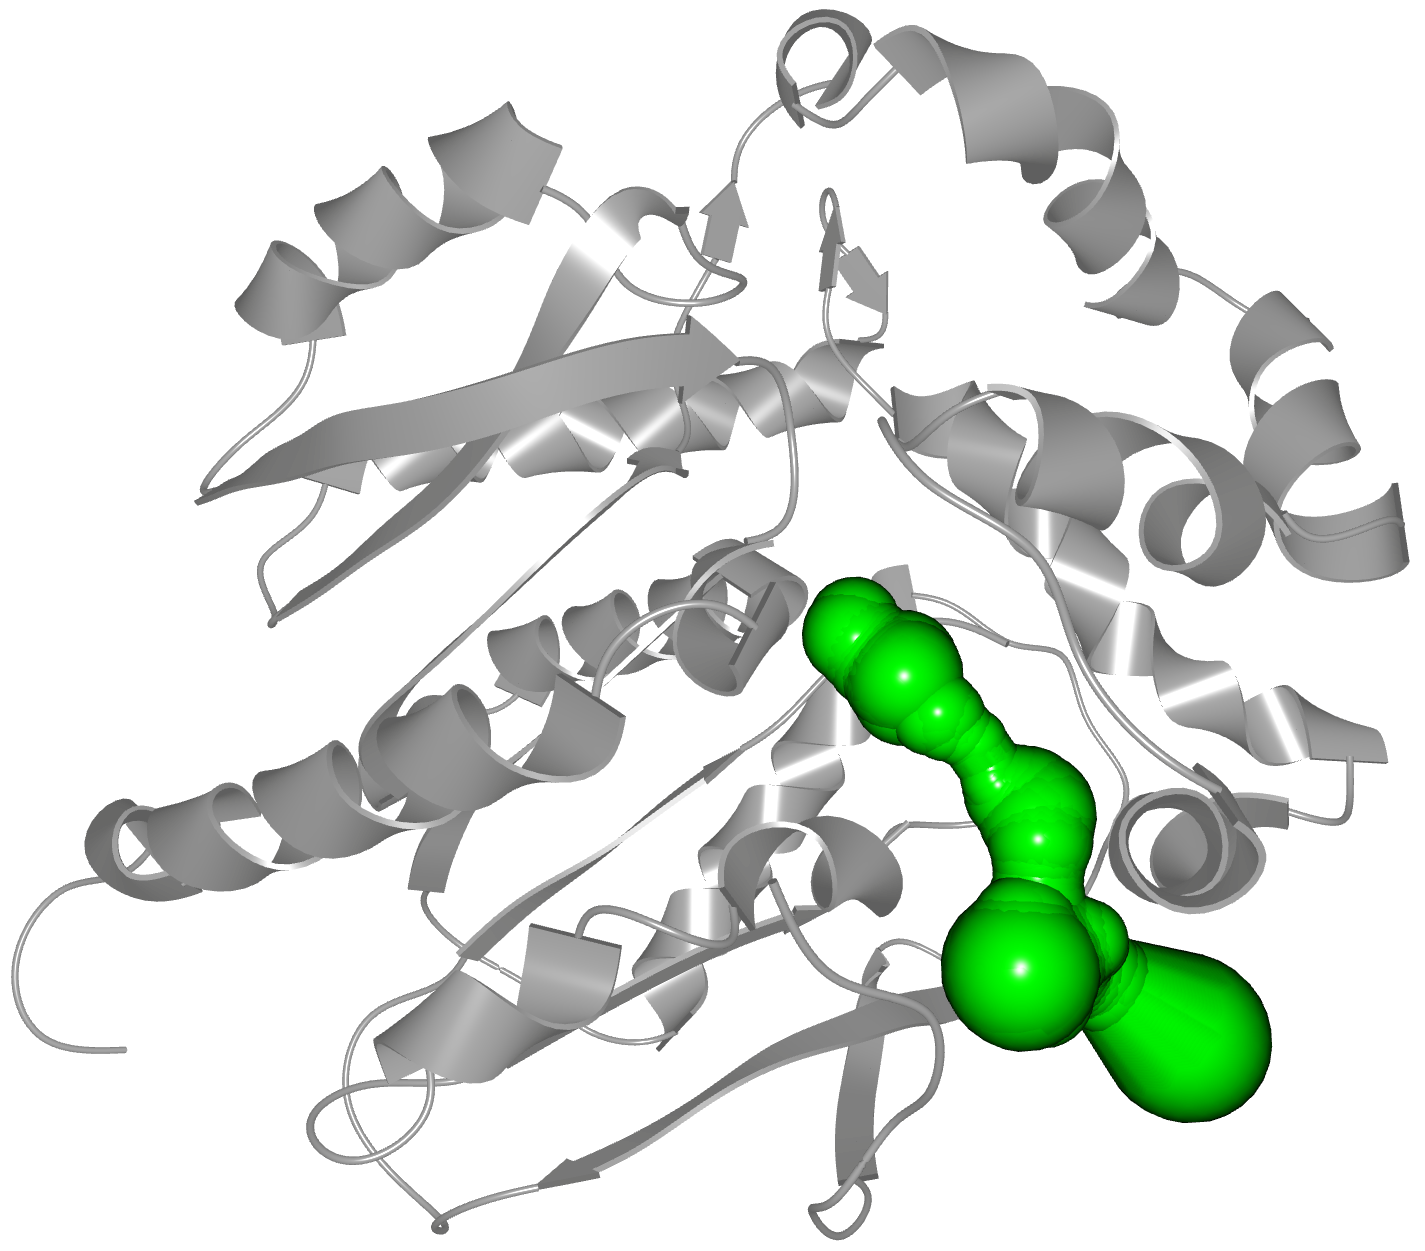
\includegraphics[width=0.38\textwidth]{fig/protein-tunnel-gray} &
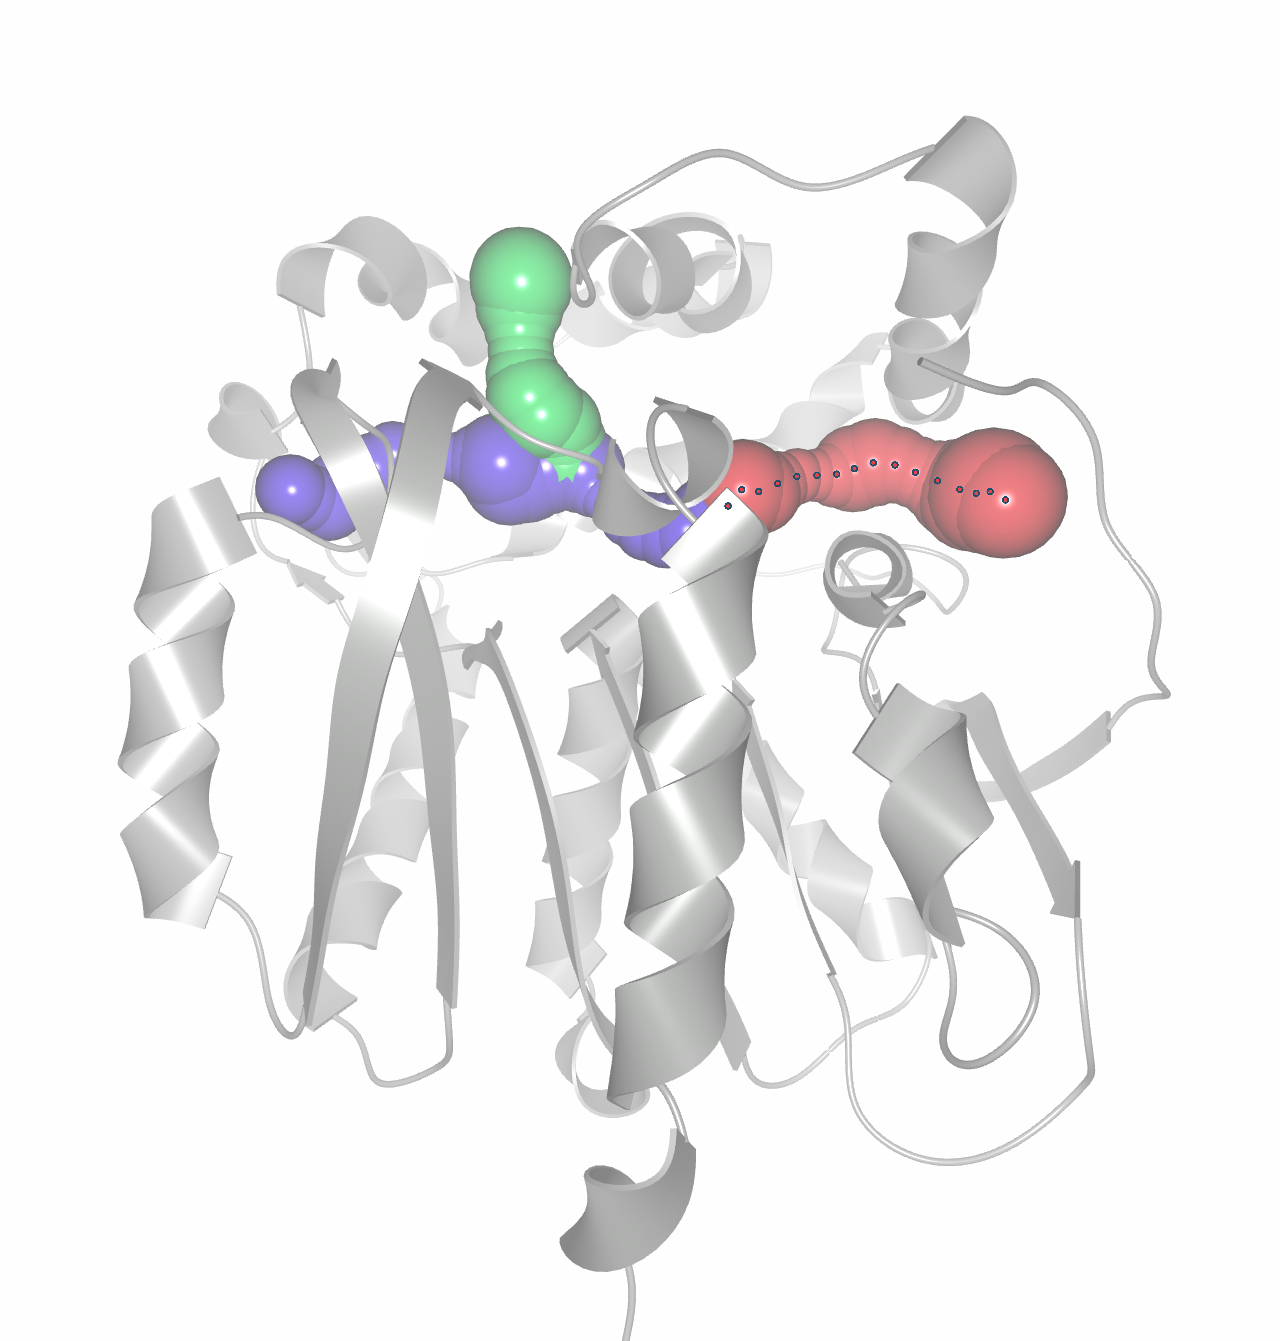
\includegraphics[width=0.3\textwidth]{fig/t05proteintunnels} &
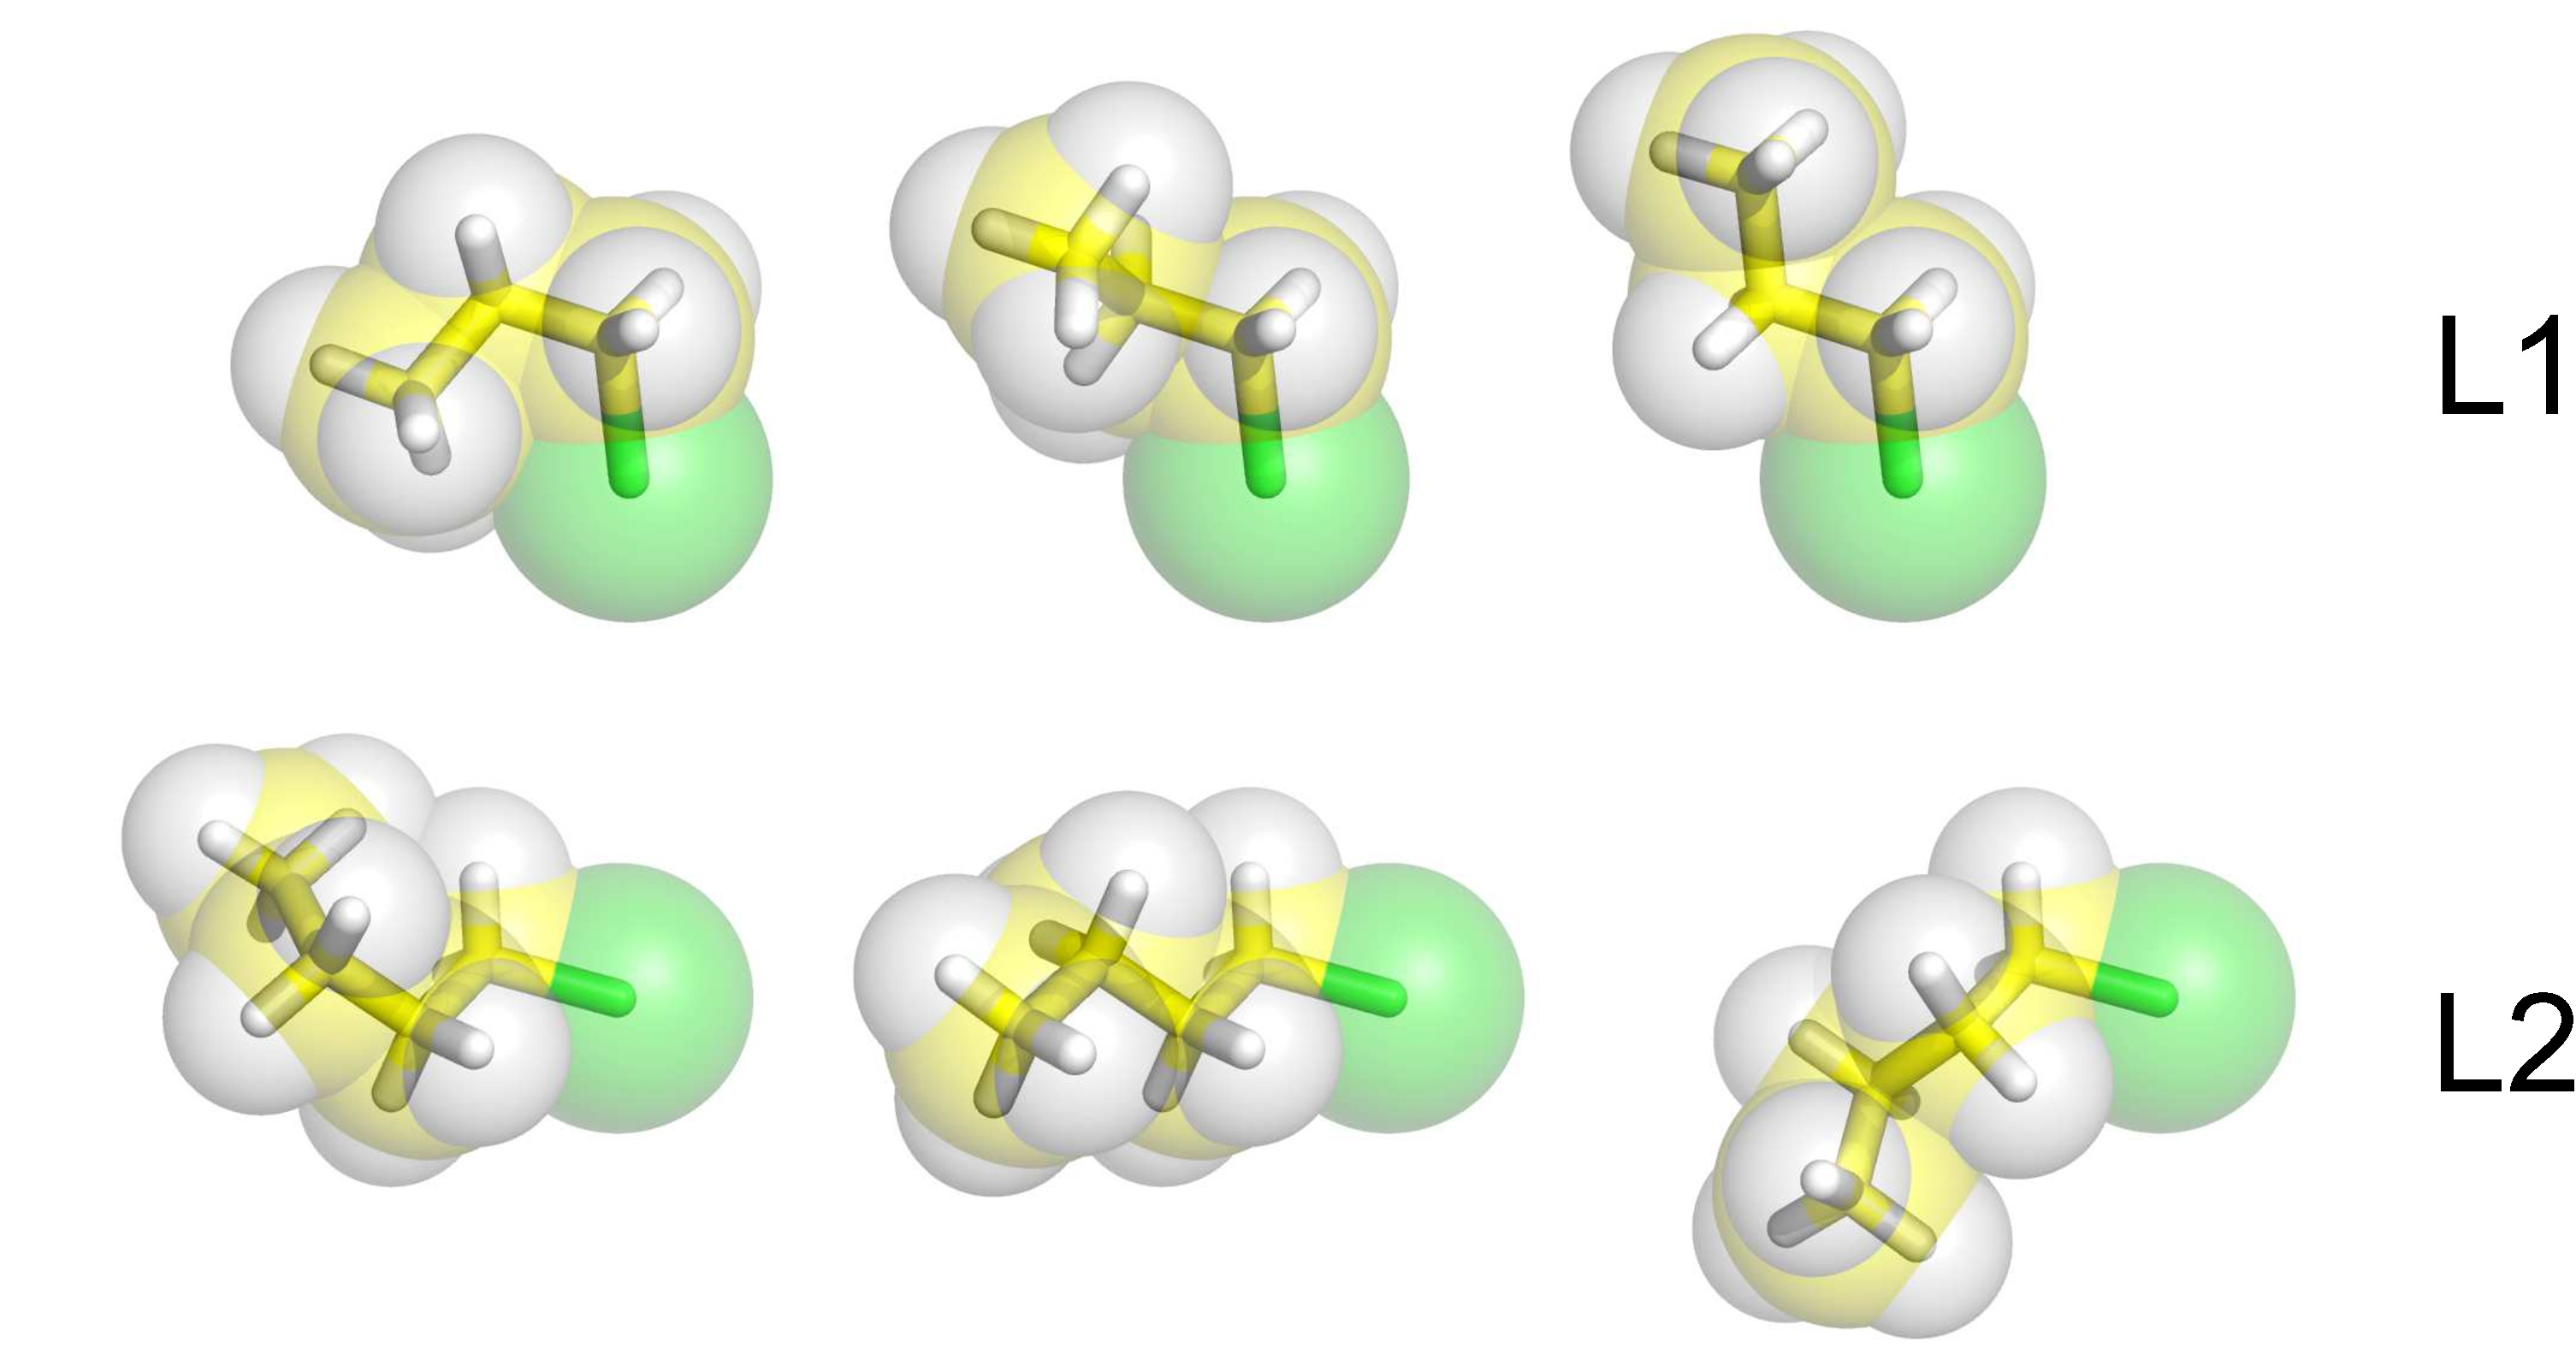
\includegraphics[width=0.45\textwidth]{fig/ligAll}  \\
(a) & (b)                        
\end{tabular}                       
\caption{\label{fig::tunnel}
    (a) The protein 1CQW visualized using the cartoon representation (gray) with 
        three tunnels (red, green, blue) detected by CAVER 3.0.
        The first tunnel is depicted red.
%        its highest ranked tunnel (green) which was detected using CAVER 3.0.
    (b) Examples of three conformations of $\LA$ (top) and $\LB$ (bottom)
}
\end{figure}



\begin{table}
\centering
\caption{\label{tab::rrt}
    Runtime and success ratio for ligand $\LA$ (left) and $\LB$ (right).
}
{
\small
\renewcommand{\tabcolsep}{1pt}
\input table.003.tex
\hskip 4pt   
\input table.004.tex
}
\end{table}





Trajectories for $\LA$ in all detected tunnels were classified as successful if they reached the last sphere of the tunnel
to distance $\dt=2$~\AA and they were considered unsuccessful otherwise.
The throughput computed from the trajectories shows that the tunnels are difficult not only around bottlenecks, but
also in other places.
The comparison of the classic bottleneck (i.e., measured by the radius of spherical probe) and throughput is depicted in Fig.~\ref{fig::tunnel2}a.
The trajectories for $\smin=0.4$ are depicted in Fig.~\ref{fig::tunnel2}b and for $\smin=0.5$ in Fig.~\ref{fig::tunnel2}c.
The successful trajectories for $\smin=0.4$ reveals that the end of the tunnel No. 3 can be approached by two different pathways.
The detail of this pathway is depicted in Fig.~\ref{fig::detail}.
Despite the low bottleneck of this tunnel, the ligand may reach its end using the alternative path way. 
This shows the strength of the analysis based on the trajectories and not only on the geometric bottlenecks.

\begin{figure}
\centering
{
\renewcommand{\tabcolsep}{-5pt}
\begin{tabular}{ccc}
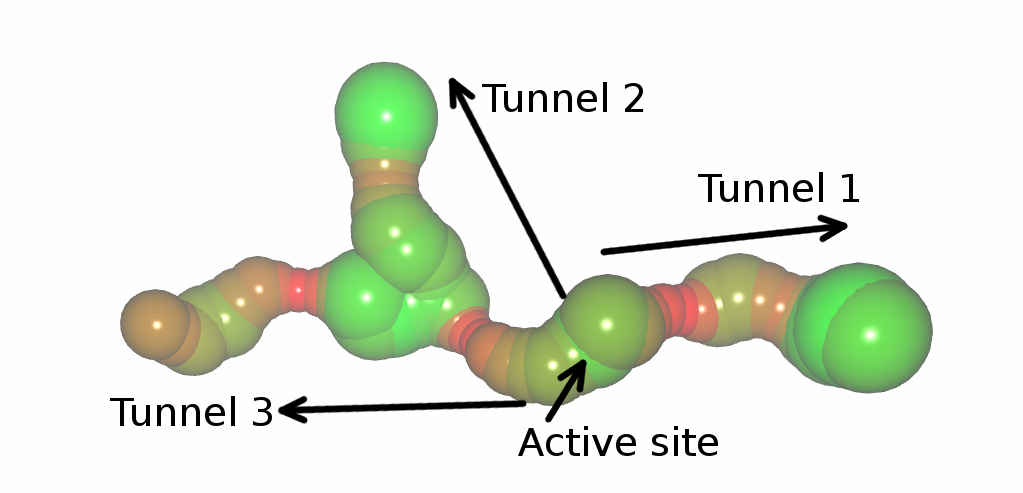
\includegraphics[width=0.38\textwidth]{fig/t05proteinBottle2T} & 
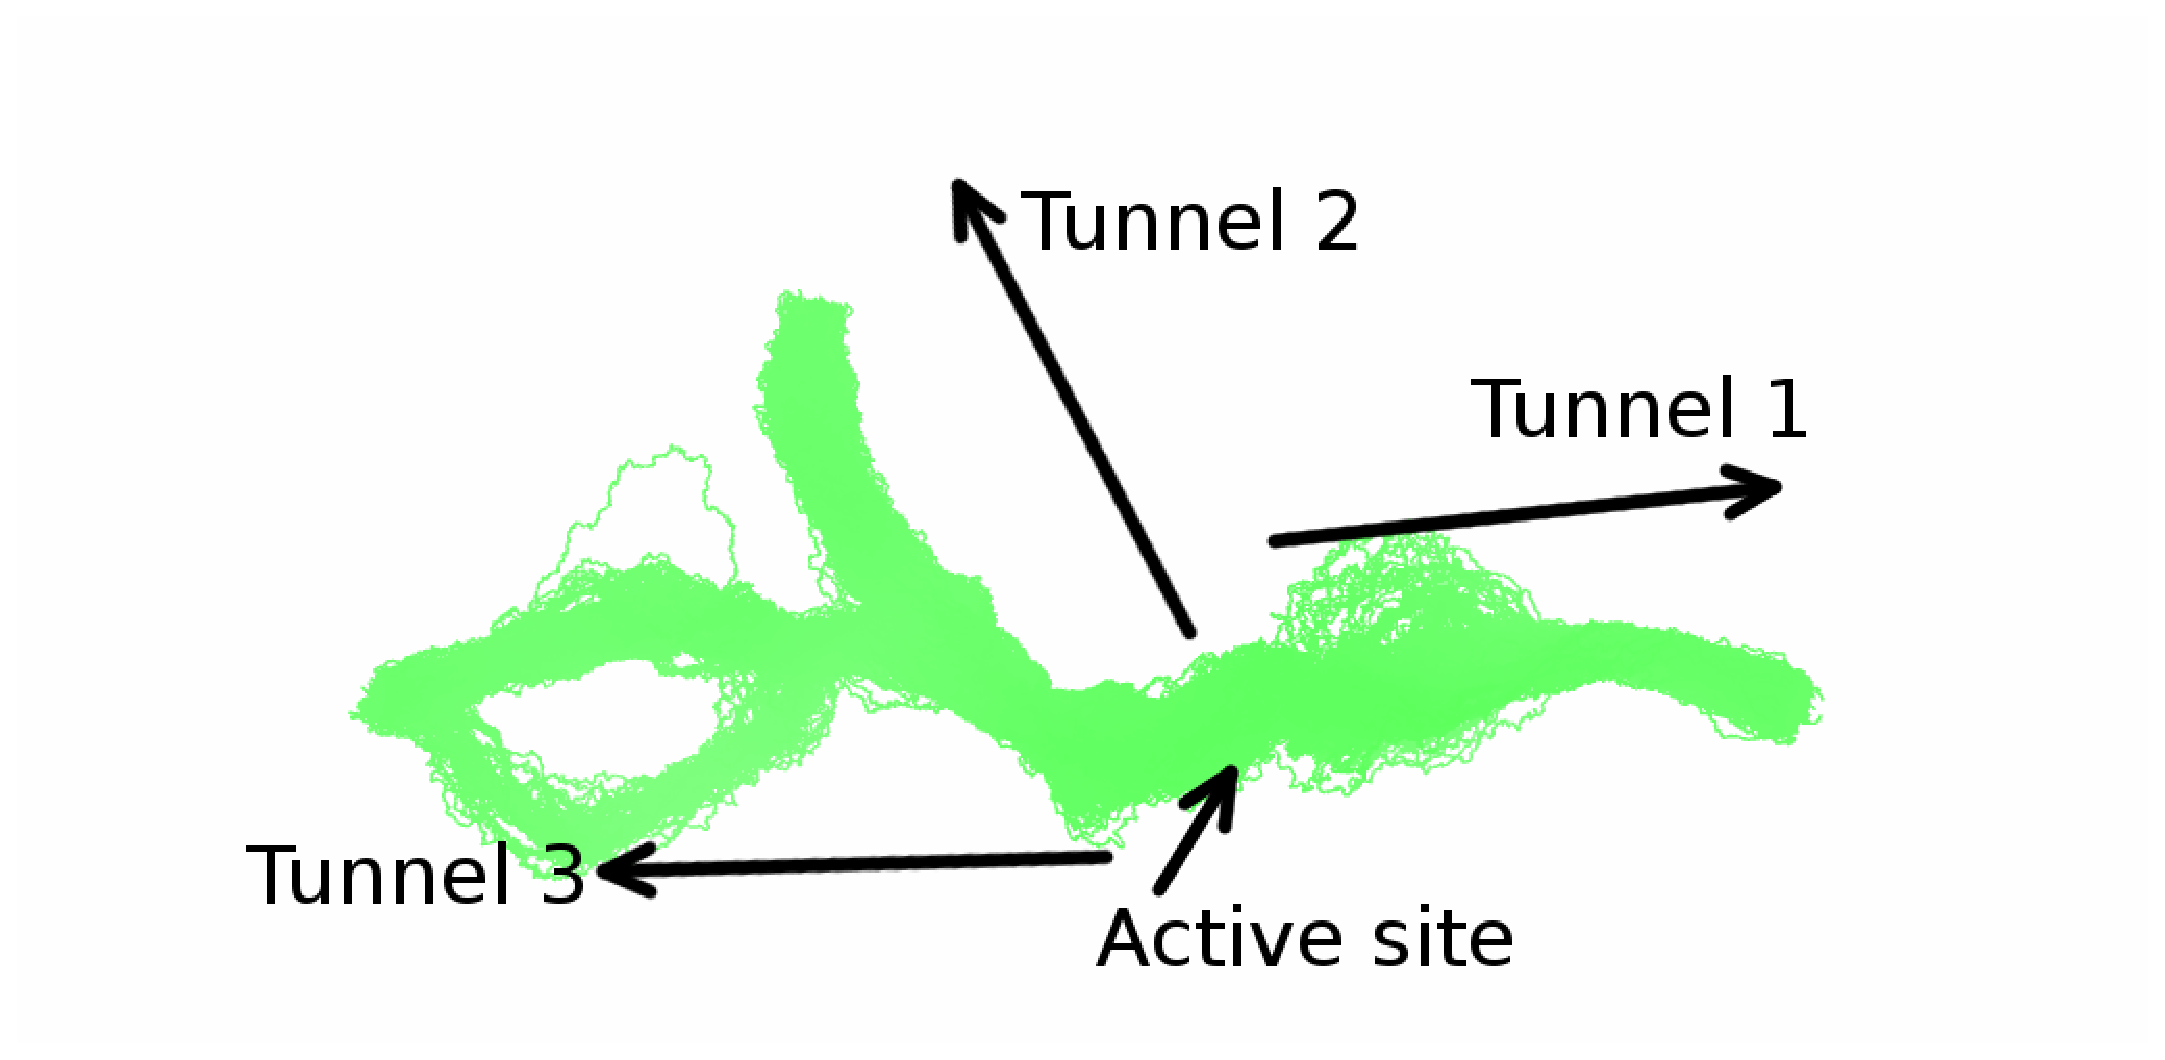
\includegraphics[width=0.38\textwidth]{fig/t04goodT} & 
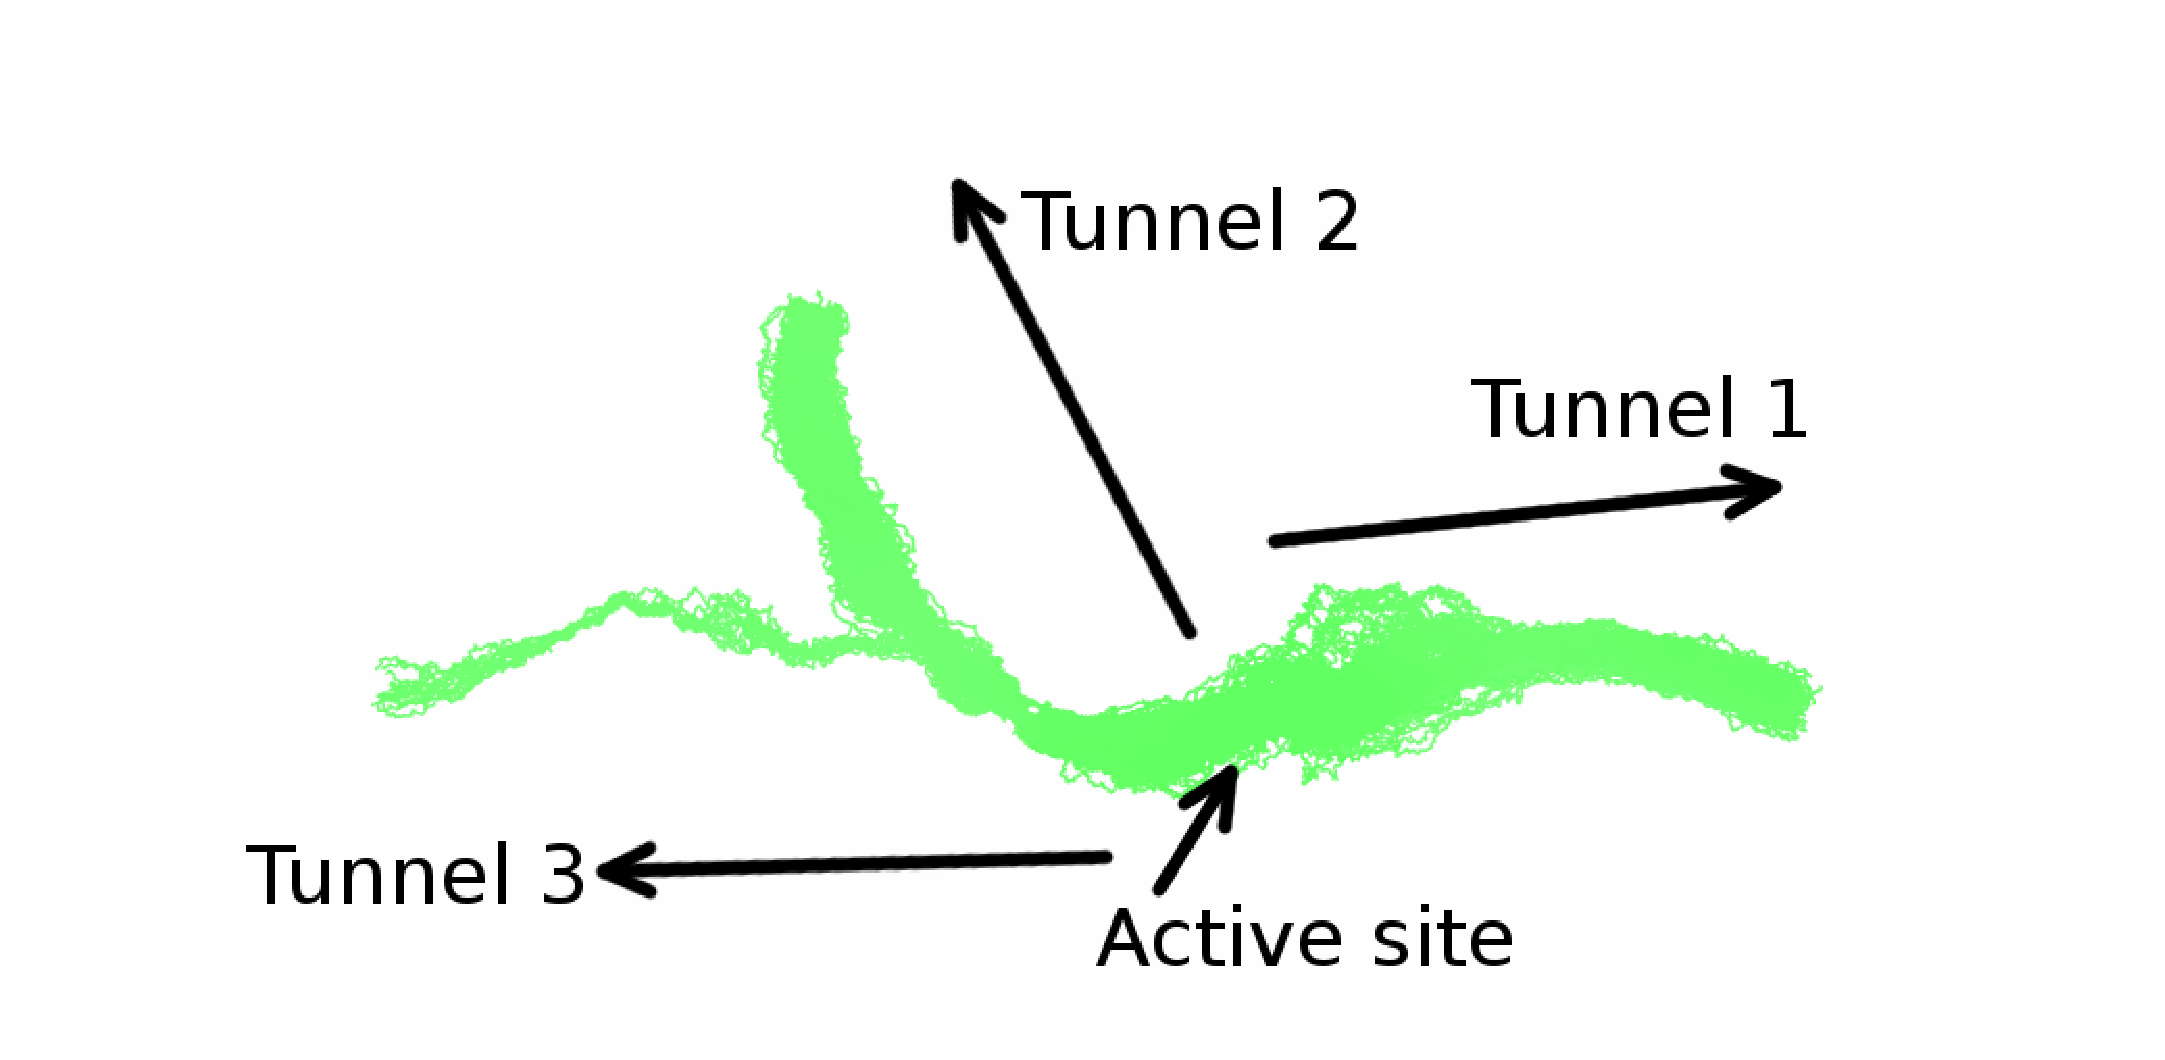
\includegraphics[width=0.38\textwidth]{fig/t05goodT} \\
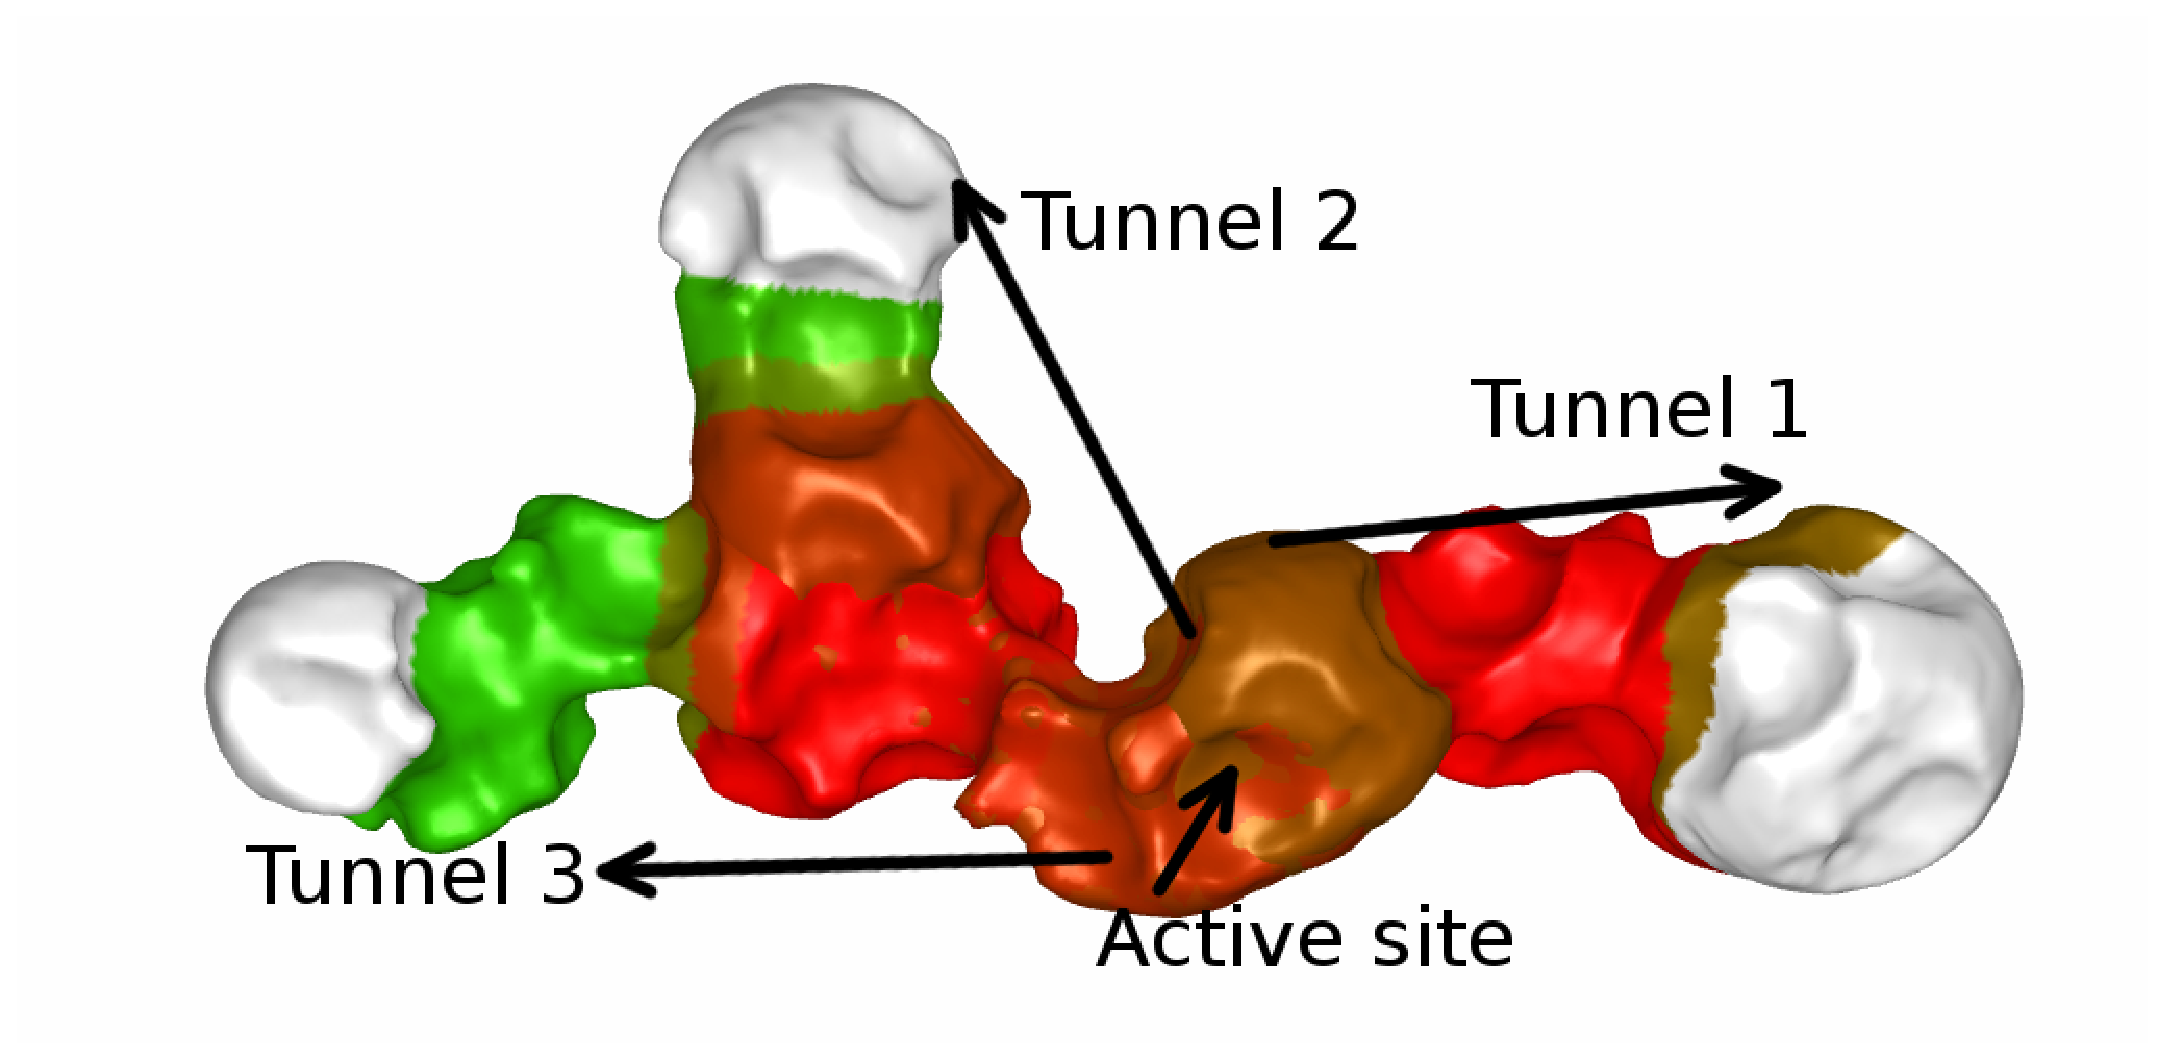
\includegraphics[width=0.38\textwidth]{fig/t05thpT} &
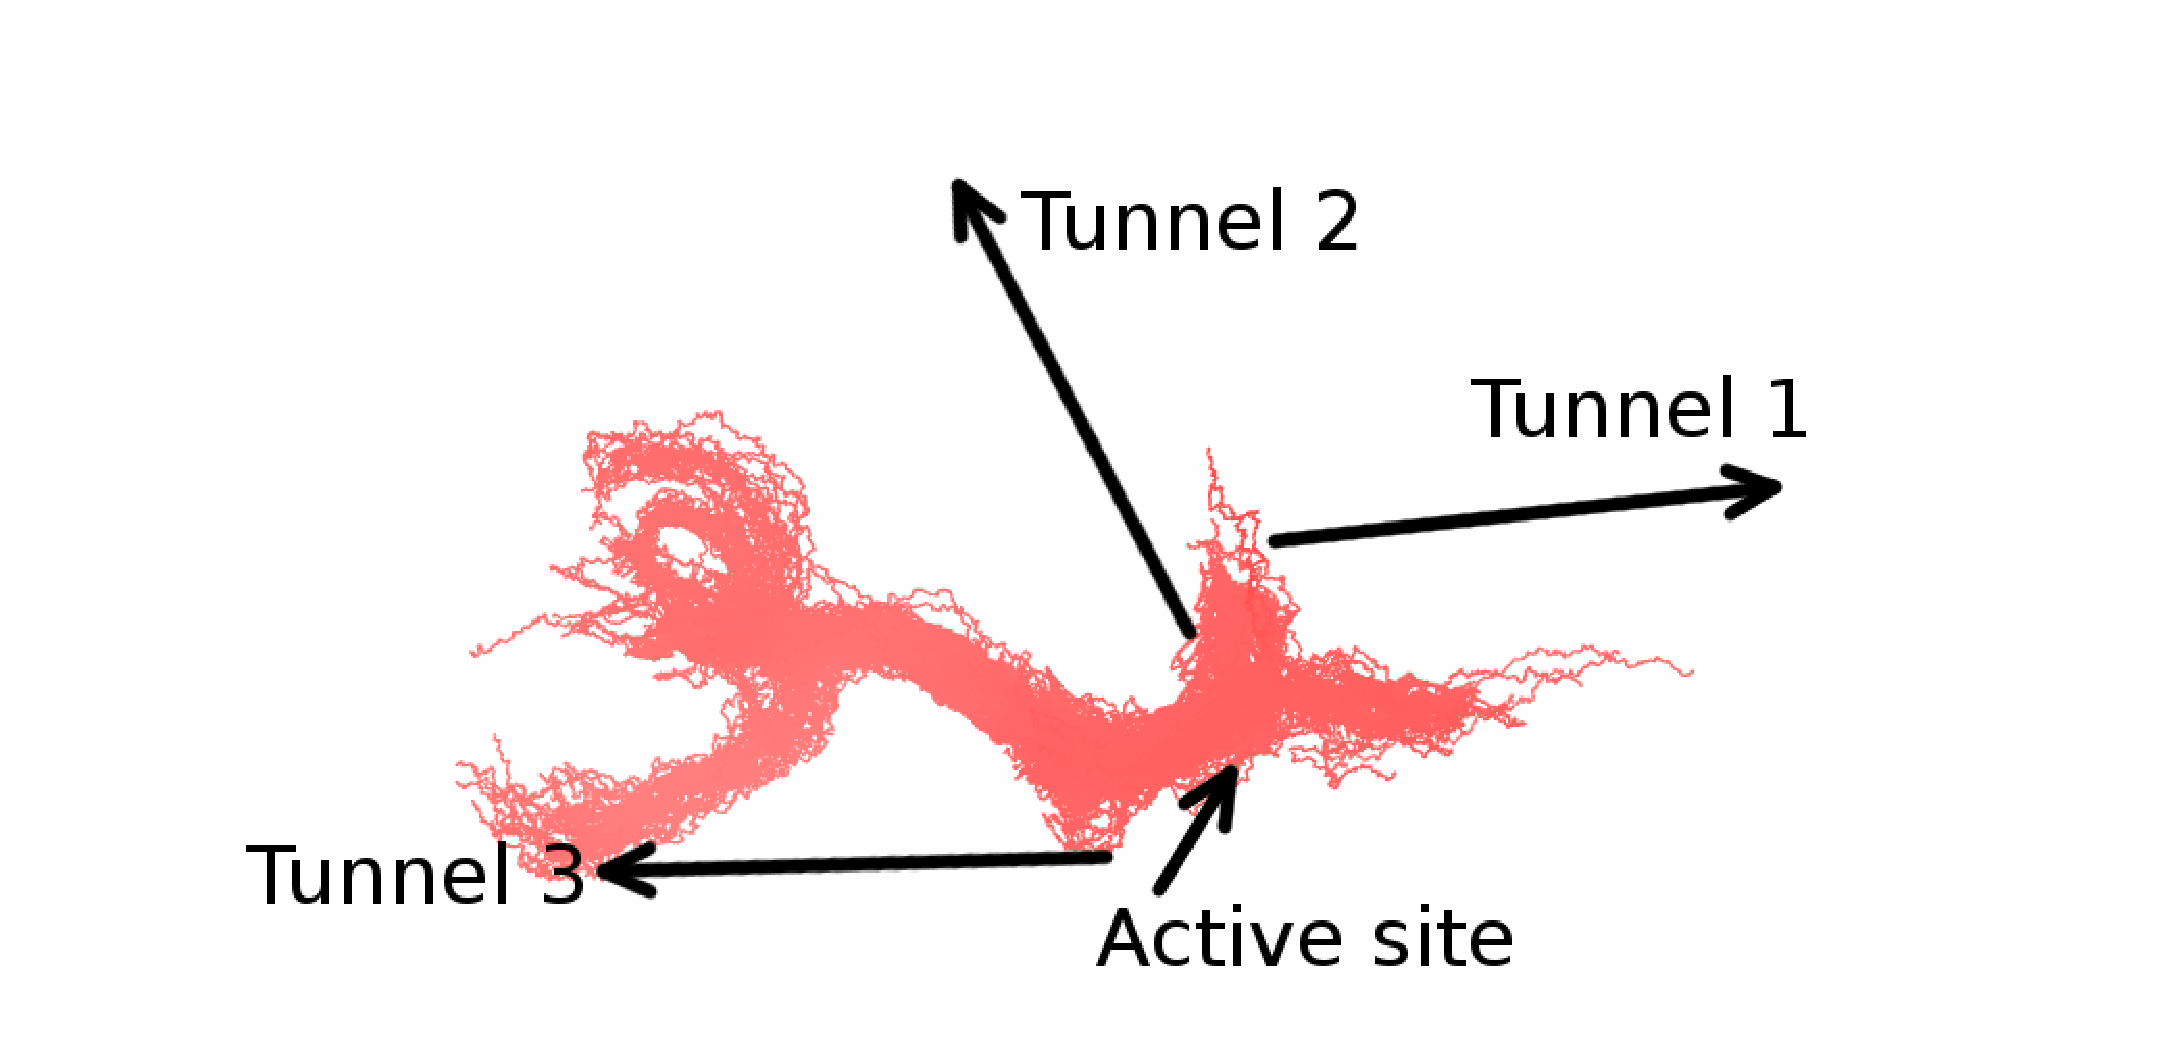
\includegraphics[width=0.38\textwidth]{fig/t04badT} &
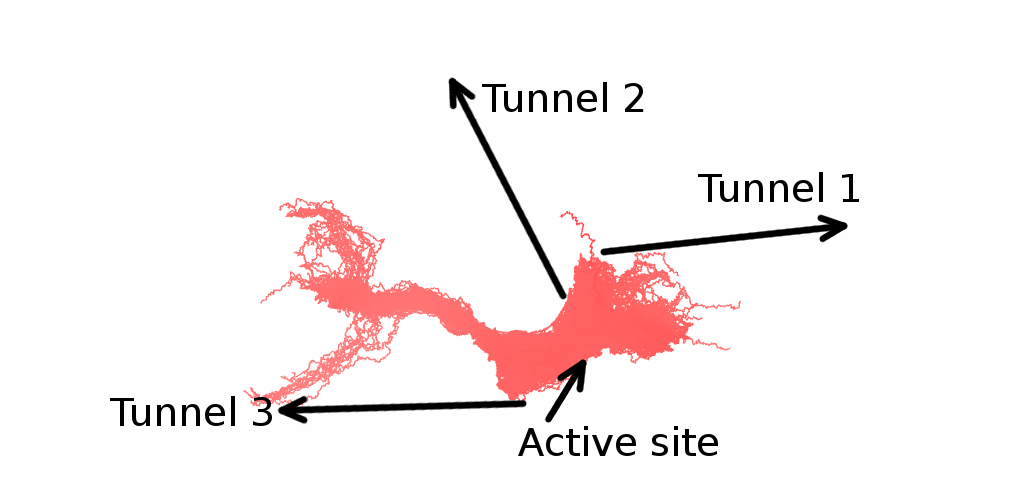
\includegraphics[width=0.38\textwidth]{fig/t05badT} \\ 
(a) & (b) & (c)                       
\end{tabular}                       
\caption{\label{fig::tunnel2}
    (a) Classic bottleneck for spherical probe (top) and visualization of throughput (bottom) for the ligand $\LA$.
    (b) Successful (green, top) trajectories that reached end points of the tunnels,
        and unsuccessful ones (red, bottom) for $\smin=0.4$.
    (c) Successful and unsuccessful trajectories for $\smin=0.5$.
}
}
\end{figure}


\begin{figure}
\centering
\begin{tabular}{ccc}
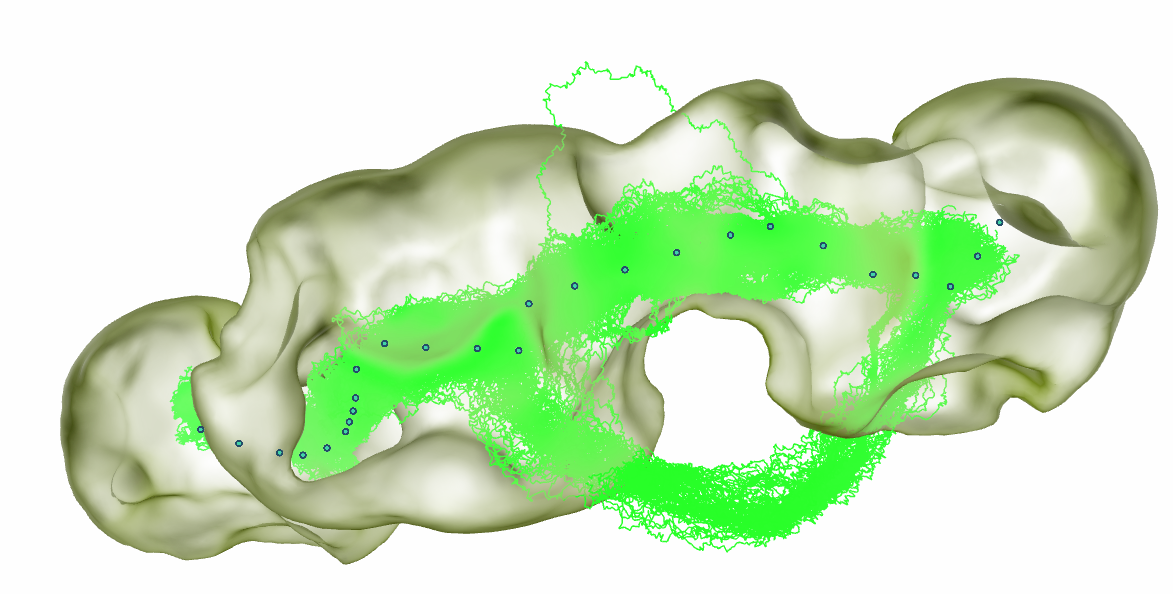
\includegraphics[width=0.32\textwidth]{fig/tunne4ac}& 
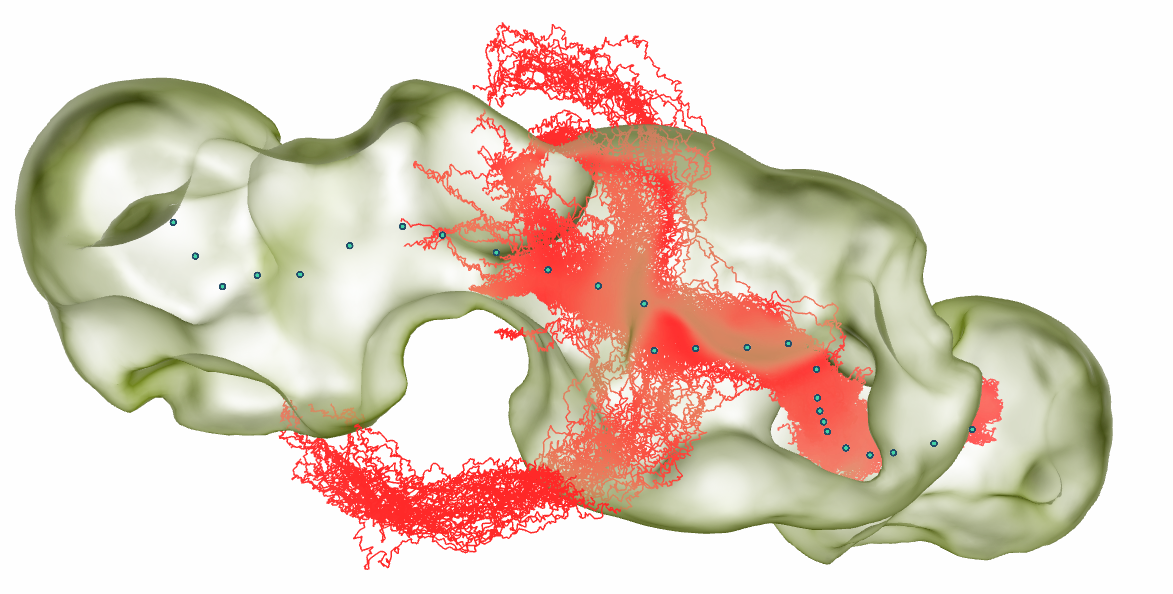
\includegraphics[width=0.32\textwidth]{fig/tunne4bc} & 
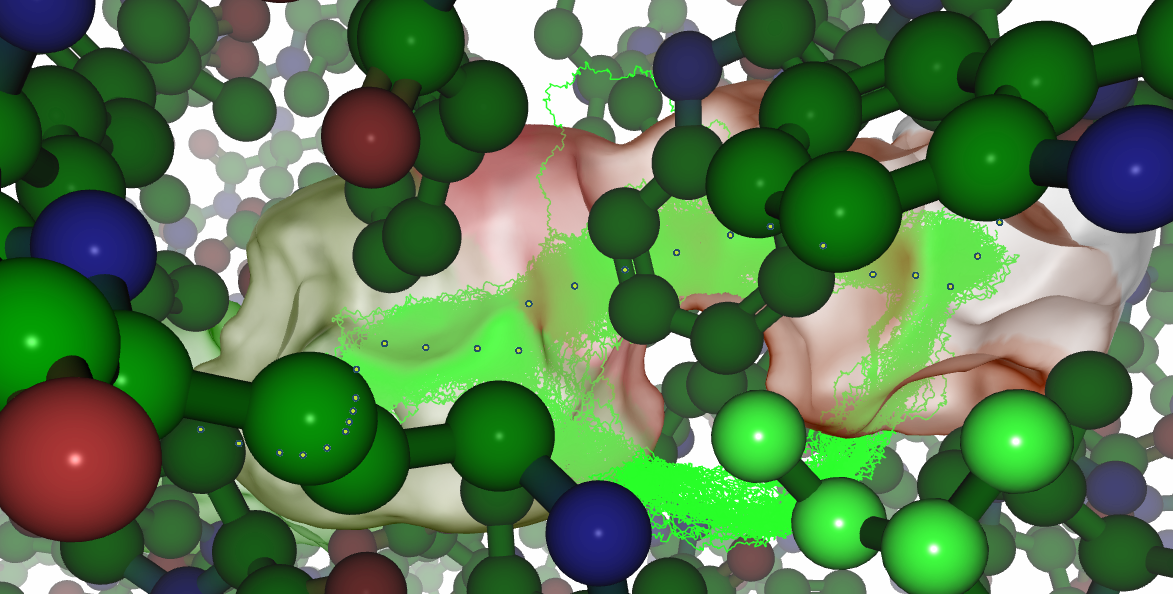
\includegraphics[width=0.32\textwidth]{fig/tunne4cc} \\
(a) & (b) & (c)                        
\end{tabular}
\caption{\label{fig::detail}
    Detailed view to alternative pathway around the third tunnel in 1CQW.
    The successful trajectories are in green (a) the unsuccessful in red (b).
    (c) Shows visualization of protein atoms around the tunnel.
}
\end{figure}





\section{Discussion}

%Trajectories computed for a ligand moving in a tunnel can reveal such properties that cannot be computed
%only based on the geometry of the tunnels.

The computed trajectories cannot be considered as `real', they should rather be considered as a hint for the biochemists.
One of the reason is that the trajectories are computed inside a static protein and static tunnels.
Real proteins are dynamic structures and consequently also the tunnels are dynamic: they move, merge or even disappear due to motions of protein atoms.
Contrary, usually static tunnels are used in protein engineering.
%multiple tunnels are detected separately in each frame of molecular dynamics and the tunnels are then aggregated to a single one.
Despite such a simplification, researches often used information about the static tunnels  to estimate the possibility of chemical reactions
at the active sites.

The second limitation is caused by the utilization of scaled-down ligands.
The protein atoms tend to fill the internal void space therefore the tunnels identified inside proteins without ligand tend
to be very narrow.
To enable at least some motion of the ligands inside such narrow tunnels, the scaling-down of the ligand atoms is necessary.
It is used also in other related tool, e.g.~\cite{cortes2005path}.
%By allowing more aggressive scaling-down, more easier a trajectory can be found.
%The tunnels therefore should be always evaluated considering various minimal scales.

Due to these reasons, the computed trajectories can be considered either as too optimistic
(e.g. because they are computed on a wide tunnel that can be in fact closed due to molecular dynamics),
or too pessimistic (e.g. the trajectory is not found because of narrow passage around the tunnel, which can be 
opened due to the molecular dynamics).
Despite these limitations, testing the tunnel traversability using motion planning technique can provide chemists more information
than the simple bottleneck radius, which is used nowadays.
For example, possible detours from the tunnel can be identified, which suggest that even a tunnel with a small
bottleneck can be traversed (Fig.~\ref{fig::detail}).

%To better utilize the results of motion planning, it is necessary to observe behavior of ligands in many simulations with various proteins.
%To the best knowledge of the authors, this is the first work attempt to analyze traversability of ligands in protein tunnels.
%Most related works, e.g. those based on motion planning, are usually focused on protein folding, or finding arbitrary pathways
%from proteins~\cite{cortes2010simulating,guieysse2008structure}.

The proposed planner is very simple and it can be improved in many ways: by using a less aggressive scaling-down technique (in order
to obtain better trajectories) or by using only a subset of conformations and a better expansion (in order to speed it up).
Having a better motion planner (in the term of the speed or even success rate) however does not automatically mean that the resulting trajectories will help the biochemists more.
The presented work shows possible advantages of the analysis based on ligand trajectories.
By comparing the planned trajectories with trajectories observed in MD simulations, thresholds for the success rate or minimal tunnel throughput can be set, which will help biochemists to make decisions.



%The runtime of the planner is currently given mainly by the collision-detection.
%As the ligand is assumed to travel only along the tunnel centerline (in the distance defined by $\rv$),
%only atoms located in the vicinity of the tunnel can be considered for collision detection.
%Fast collision-detection can be achieved either using fast hierarchical data structures as OBB (implemented, e.g., in~\cite{ozcollide})
%    or using collision-detection system developed directly for proteins~\cite{ruiz2005biocd}.
%We assume that a conformation $l \in \L$ can be switched to all other conformations in $\L$.

%parmas:
%$\RI$
%$\rv$
%$\dt$
%The presented expansion procedure favors the samples with maximal scale (they are tested first), the trajectory contains samples with higher scales at the easy part of the tunnels (e.i., wide areas), and the smaller scales are used only if the ligand has to fit into a narrow space.



\section{Conclusion }
%In the future, we will focus on the following extensions proposed by the domain experts.
%Only ligand flexibility is included in the current algorithm but the flexibility of amino acid side-chains would greatly improve the prediction. 
%Moreover, incorporation of some scoring function for energy evaluation would introduce the characterization of not only geometrical but also physico-chemical properties and would further improve the prediction ability of our approach.

Protein tunnels are transporting pathways for ligands towards active sites.
In this paper, we propose to analyze the traversability in the tunnels using motion planning, that can consider both shape
of the protein and ligand.
We proposed modifications to the RRT method to compute trajectories for a ligand represented by a library of common conformations.
The corresponding configuration space is sampled using the guided sampling, where a virtual sphere moves along the tunnel and attracts growth
of the tree towards it.
To enable trajectory computation in narrow tunnels, atomic radii of the ligand are scaled down.
Computed trajectories allows us to evaluate the traversability of the tunnels using
accessibility, throughput and also by visualizing typical pathways found by the planner.
These properties can help to better understand importance of the tunnels.

%which can be useful in the virtual screening



\bibliographystyle{plain}
\bibliography{paper}

\end{document}











% ======================================================================
%
%    UNUSED TEXT      UNUSED TEXT      UNUSED TEXT     UNUSED TEXT
% ======================================================================




%RRT--Retraction~\cite{zhangRetraction} improves sampling in the narrow passages by retracting the newly added configuration
%closer to obstacles.
%%for motion planning of 3D objects.
%After $\qrand$ is generated and its nearest neighbor $\qnear\in \T$ is found, the segment from $\qrand$ to $\qnear$ is checked for collision.
%The tree is extended normally if the segment is free, otherwise the retraction step is performed.
%The task of the retraction step is to find a contact configuration  that minimizes the distance to $\qrand$.
%The contact configuration $q$ is found on the line and its neighborhood is searched to find another contact configuration $q'$ such that 
%$\varrho(q',\qrand) < \varrho(q,\qrand)$.
%The retraction is terminated after predefined number of steps or if no new contact configuration can be found.
%%The configuration trees built by RRT--Retraction can therefore contain more nodes than is the number of planning iterations,
%as the tree can be expanded by upto $\Nrret$ contact configurations in each iteration.
%An example of the retraction is depicted in Fig.~\ref{fig::rrtretraction}.
%The RRT-Retraction was designed for path planning of 3D objects, where the straight-line local planner is used to connect two configurations, which allows us to find the contact configurations by random sampling.
%The RRT--Retraction can quickly penetrate to narrow passages, but its computational burden is significantly
%increased due to necessity to find the contact configurations.
%The method was designed mainly for 3D path planning, but it can be combined with other planners
%for motion planning of many-DOF robots~\cite{pan2010retraction}.
%    e.g. for articulated robots~\cite{pan2010retraction}.
%RRT--Retraction combined with decomposition-based path planners for articulated robots with many DOF was proposed in~\cite{pan2010retraction}.

%The narrow passage problem has been studied intensively 
%Due to its low volume, the probability of expanding the nodes towards the passage is small~\cite{hannaWIS}.
%    many iterations are needed before a tree can be built through the passage~\cite{hannaWIS}.
%Recently, we have proposed a novel method for tunnel detection using sampling-based motion planning, namely using Rapidly Exploring Random Tree (RRT) method~\cite{vonasek2016application}.
%In comparison to existing approaches~\cite{Petrek20071357,petrek2006caver}, this RRT-based approach~\cite{vonasek2016application} 
%handles the dynamics without need to cluster and match Voronoi diagrams from consecutive frames.

%We further consider a spherical probe $\Sprobe$  of radius $\probe$ encapsulating the ligand.
%Let $q=(x,y,z)\in\C$ denote the configuration (position) of the probe, where
%the configuration space $\C$ consists of all possible configurations.
%For each configuration $q\in\C$ we assume, that its largest collision-free radius $r(q) \in \mathbf{R}, r(q)\ge 0$ can be computed, e.g.
%using collision detection.
%using collision detection.
%Let $L(q) \subseteq \mathbf{R}^3$ denote the geometry of the ligand at position $q \in \C$.
%Similarly to geometry of molecule, the geometry of ligand is union of hard sphere model.
%A probe is represented by one sphere of radius $\probe$.
%The collision-free region $\CF \subseteq \C$ is formed by configurations, where $\Sprobe$ can be placed without any collision, i.e., 
%$\CF = \{q \in \C | \Sprobe(q) \cap \SS = \emptyset\}$, where $\Sprobe(q)$ is the sphere with radius $\probe$ at configuration $q$.
%The distance $\dist(q_1,q_2)$  between two configurations $q_1,q_2\in\C$ is measured using 3D Euclidean metric.

%This radius can be detected using collision detection method.
%The configurations outside the protein $\CG \subseteq \C$ are collision-free with sphere $\Sgprobe$ of radius $\gprobe$, $\gprobe> \probe$,
%$\CG=\{q\in \C| \Sgprobe(q) \cap \SS = \emptyset \}$.
%A configuration $q \in \CG$ is referred to as {\sl goal configuration} in the rest of the paper.
%By computing $\alpha$-shape of the molecule, we can identify atoms located at the surface. 
%These atoms are referred to as {\sl surface atoms} in the rest of the paper.
%The distance between a configuration $q \in \C$ and its nearest surface atom is referred to as $\dists(q)$.
%We assume, that for each configuration $q$, the largest collision-free radius $r(q)$ can be computed.
%Let $r(q)$ denote the radius of the largest collision-free sphere at configuration $q$.

%Dynamic proteins are represented by a sequence of $n$ snapshots (frames).
%The tunnels change with the protein dynamics as well: their width and position change, they can merge with other tunnels or even disappear.
%The free region $\CF$ is therefore different in each frame, as positions of atoms change.
%For the sake of simplicity, a single notation $\C$ resp. $\CF$ is used in this paper and it is valid for the frame being processed.



%sampling-based for 
%protein-ligand access and docking \cite{bayazit2001ligand,singhLig,apaydin2004stochastic,cortes2010simulating}
%protein and RNA folding~\cite{amatoPF1,ApaBru03}
%protein loop motions~\cite{cortes2004geometric},
%domain motions~\cite{kirillova2008an}, 
%and motions of pairs of alpha-helices in transmembrane proteins~\cite{enosh2007prediction}

%The tree is extended from a node, that is selected as a nearest node to a randomly generated configuration in the configuration space.
%The highest probability of expansion have nodes with large Voronoi cells. 
%Due to this Voronoi-bias, the tree grows towards unexplored regions of the configuration space.
%However, the Voronoi-bias brings disadvantages in narrow passages.
%nodes in the narrow passages.



%The behavior of RRT in the narrow passages was analyzed using Voronoi diagrams in~\cite{yershovaDDRRT}.
%The nodes in the tree can be divided into two groups: frontier nodes, whose Voronoi cells grow together with growth
%of the environment and boundary nodes, which are close to the obstacles. %~\cite{yershovaDDRRT}.
%The tree cannot be expanded from the boundary nodes.
%In a narrow passage, the nodes are both boundary and frontier.
%These nodes are frequently selected for the expansion, because they are the frontier nodes, however the tree cannot be expanded
%from them, because they are also the boundary nodes. 
%To suppress selection of the boundary nodes, authors of~\cite{yershovaDDRRT} suggest to define an action radius around each node.
%The node is selected for the expansion only if its radius is larger than the distance to the random sample.
%The radius of new nodes is set to $\infty$ and it is decreased to a predefined value $\rdd$ if the node cannot be expanded.
%A Dynamic-Domain strategy for RRT (RRT--DD) is proposed in~\cite{yershovaDDRRT}:
%each node holds an action radius defining how far can be a random sample $\qrand$ that activates the node for the expansion.
%The RRT--DD algorithm generates random samples $\qrand$  and finds its nearest neighbor in the tree
%$\qnear$ until $\rho(\qrand,\qnear) < \qnear.radius$. 
%Although the algorithm is efficient in the narrow passages, it is strongly influenced by the parameter $\rdd$.
%To decrease the sensitivity of the method to the parameter $\rdd$, it can be automatically adjusted, which
%was proposed in RRT--ADD (RRT with Adaptive Dynamic Domain)~\cite{jailletATDDRRT}.
%Another schema to automatically adjust parameters of the RRT-based planners was proposed in~\cite{schneider2015completely}.

%Retraction-RRT~\cite{zhangRetraction} generates random samples uniformly as in the original RRT, but it
%attempts to shift them into the narrow passages.
%A~random configuration $\qrand \in \CF$ is generated and a close non-free configuration $q \in \CO$ is found. 
%A~contact configuration $q_c$ on a segment $(\qrand,q)$ is found and its neighborhood is searched for
%$q_c'$ minimizing the distance between $q$ and $q_c'$. 
%The configuration $q_c'$ is then added to the tree.
%It was shown that this approach can deal with narrow passages efficiently,
%because the generated contact configurations penetrate into the narrow passages.
%However, to find the contact configurations, the collision detection algorithm is called frequently, which can decrease
%the performance of the algorithm.

%The goal-bias principle can be further extended by sampling the configuration space along a path computed in the workspace~\cite{vonasek2009rrt,amatoOBRRT}.
%%Geometric path in the workspace~\cite{vonasek2009rrt} or medial axis of the 3D space~\cite{amatoOBRRT} can be used to guide the tree.
%Sampling along geometric paths constructed in the workspace is suitable for low-dimensional configuration spaces, e.g. for
%path planning of mobile robots.
%However, the geometric paths computed in workspace are less effective for sampling in high-dimensional configuration spaces~\cite{hannaWIS}.
%



%of the narrow passages is related to narrow passaged of the workspace~\cite{hannaWIS}.
%
%is to manipulate the random samples, e.g. to change their rotation, rotation or both parts or to shift them closer to the medial
%axis of the workspace~\cite{amatoOBPRM}.

%In~\cite{amatoOBPRM} several strategies for validating non-free random samples have been proposed.
%Authors propose different manipulation procedures for random configurations generated during the learning phase.
%For example, the random configuration can be placed into the roadmap with changed rotation, translation or both, or it can be
%shifted away from an obstacle allong a line connecting the sample and medial axis of the obstacles.
%In a configuration is invalid, it is pushed randomly into various directions to gen free samples around boundaries of $\CO$.





% ===============================================================================


%25\% of VDW radii, T-RRT \cite{jaillet10costmap}

%\red{The tunnel detection task differs from classic motion planning it two main aspects: a) the goal configuration
%is not explicitly defined, and b) multiple pathways (tunnels) should be detected.}


%Molecular structures can be represented as articulated bodies and sampling-based methods can be used
%Path planning methods have been used to expore the conformational space of 
%proteins~\cite{novinskaya2015improving,songPFintro,mollProt,proteinRRT},
%Other applications of sampling-based approaches is in detection of 
%folding pathways~\cite{amato2002using}, analyzing protein loops~\cite{cortes2004geometric}, 
%or modeling large-scale transitions in a protein structure~\cite{raveh2009rapid}
%The geometric-based tunnel detection approaches provide fast computation of tunels in large protein structures and they
%have been integrated in several tools like Caver~\cite{bara2014caver}, Chexvis~\cite{masood2015chexvis} and other.
%Most of the proposed methods consider only spherical models of ligand~\cite{benkaidali2014computing}.

%dxTuber: Detecting protein cavities, tunnels and clefts based on protein and solvent dynamics:
%furtng protein cavities, tunnels and clefts based on protein and
%solvent dynamics insights into the protein in question. For example, empty
%space in a protein structure can provide valuable insight into protein properties such as internal hydration, structure stabilization,
%substrate translocation, storage compartments or substrate binding sites [1,2]. This information can be visualized by means of cav-
%ity analysis. Over the years numerous cavity detection tools have been developed including [3–17] that depict cavities either directly
%[3–6,8,10–17] or indirectly by identifying lining residues [9] or filling a cavity with water molecules [7]. The main strategies used
%in these geometry-based algorithms [1] can be grouped into four categories plus combinations of these.
%n the motion planning problem, that is widely studied in robotics, the task is to find a feasible trajectory for a robot between two

%given positions in an enironment.
%To utilize the motion planning approaches, the ligand is considere as the robot and the protein's atoms as the obstacles.
%Computing feasible (traversable) tunnels for non-spheric ligands requires to consider also rotations of the ligands, which 
%can be solved using sampling-based approaches like Probabilistic Roadmaps (PRM)~\cite{kavrakiPRM} or Rapidly Exploring
%Random Trees (RRT)~\cite{lavalleRRT}.
%Sampling-based methods randomly samples configuration space of the robot (ligand) and the samples are classified
%as free or non-free using collision detection.
%The free samples are stored in a graph structure.
%A path in the grap then corresponds to a motion in the workspace.



%In~\cite{guieysse2008structure}, RRT method is used to compute pathways for flexible ligands.


%\cite{lindow2012dynamic}
%Analysis of protein dynamics suggests that internal cavities and channels can be rather dynamic structures. 
%Voronoi-based algorithm to extract the geometry and the dynamics of cavities and channels from a molecular dynamics trajectory.
%The algorithm requires a pre-processing step in which the Voronoi diagram of the van der Waals spheres is used to calculate the cav-
%ity structure for each coordinate set of the trajectory. 
%In the next step, we interactively compute dynamic channels by analyzing the time evolution of components of the cavity structure. Tracing of the
%cavity dynamics is supported by timeline visualization tools that allow the user to select specific components of the cavity structures
%for detailed exploration. All visualization methods are interactive and enable the user to animate the time-dependent molecular struc-
%ture together with its cavity structure. To facilitate a comprehensive overview of the dynamics of a channel, we have also developed a
%visualization technique that renders a dynamic channel in a single image and color-codes time on its extension surface. 
%
%
%Sampling-based motion planning algorithms from the field of robotics have been very successful in exploring the
%conformational space of proteins
%\cite{novinskaya2015improving}
%Sampling-based algorithms explore the conformational space of a protein by randomly sampling it (usually using a special
%heuristic) and constructing a graph where each node represents a feasible low-energy protein conformation (or state), and each
%edge represents a possible low-energy local transition between two states. 
%The computed graph describes the topology of a protein’s energy landscape and the connectivity of its lowenergy areas. 
%This graph can be used to find possible large-scale transitions between two given protein conformations.
%

%Sampling-based methods have been very effective for the fast computation of representative motions of molecular systems \cite{al2012motion, gipson2012computational}


%A broad range of approaches exploit sampling-based techniques to address various biological problems, such
%as exploring energy landscapes \cite{devaur2014sampling} ,
%modeling protein folding pathways \cite{amato2002using}, analyzing protein loops \cite{cortes2004geometric}, 
%or modeling large-scale transitions in a protein structure \cite{raveh2009rapid}

%In computational biology, molecules and proteins are modeled as articulated bodies and sampling based planners are used to simulate
%protein folding and protein-ligand interactions  \cite{al2012motion} 
%asi spis necitovat \cite{gipson2012computational}



%Ms have been applied to model molecular motions by modeling the molecule as an articulated linkage and 
%replacing the typical collision detection validity check with some measure of physical viability (e.g., potential energy).
%Protein motions, ranging from molecular flexibility to large-scale conformational change, play an essential role in many biochemical processes. 
%!!to map transitinos between specific conmfotrmations!!!!
%ample conformation space more effectively, and we describe extensions of our framework to automate
%the process and to map transitions between specified conformations.
%\cite{thomas2006simulating}
%

%In subsequent work, our group used another PRM variant on this problem \cite{bayazit2001ligand}
%Our group was the first to adapt PRMs to model protein folding pathways 
%\cite{amato2003using, amato2002using, song2003apath}

%Using a standard modeling assumption for proteins that bond angles and bond lengths are fixed \cite{sternberg1996protein}, 
%the only dof in our model are the backbone’s phi and psi torsional angles which are modeled as revolute joints with values 0 .. 2pi

%
%The roadmap produced by our technique is an approximation of the protein’s energy landscape. 
%Roadmap quality is measured both by how realistic (as compared to experimental data) its pathways are and by how many samples are required
%to achieve the desired accuracy. 
%The latter is important because it determines what size molecules can be analyzed.
%Hence, sampling is the key to producing a good approximation of the land-scape. 
%Note that only a relatively small portion of the conformation space ‘near’ the target conformation(s) is of interest in modeling motions. 
%This implies that we should use biased sampling to cover the regions of interest efficiently.
%
%genrovani lepsich vzorku: using rigidity analysis~\cite{thomas2006simulating}
%or perturbing:
%iterative sampling process where we apply small Gaussian perturbations to existing conformations~\cite{amato2003using, amato2002using, song2003apath}
%
%rrt for tunnel (pathway) detection
%\cite{cortes2010simulating}
%\cite{corset2005path}
%\cite{guieysse2008structure}
%

%Many modifications have been proposed for RRT to speed up the growth of the tree~\cite{kuffnerRRTC}, 
%     to consider an optimality criteria such as path length~\cite{karaman2011sampling}, and to improve behavior in narrow passages~\cite{amatoOBRRT,vonasek2009rrt,zhangRetraction,schneider2015completely}. 
%For example, RRT--Retraction~\cite{zhangRetraction} analyzes the line segment from $\qnear$ to $\qrand$.
%If the line segment is collision-free, the tree is expanded normally using the straight-line planner.
%Otherwise, the contact configuration on the line segment is constructed and its neighborhood is searched
%for other contact configurations in order to minimize the distance to $\qrand$.
%This retraction step allows RRT--Retraction to place the nodes of the tree into narrow passages.



%The behavior of RRT in the narrow passages was analyzed using Voronoi diagrams in~\cite{yershovaDDRRT}.
%The nodes in the tree can be divided into two groups: frontier nodes, whose Voronoi cells grow together with growth
%of the environment and boundary nodes, which are close to the obstacles. %~\cite{yershovaDDRRT}.
%The tree cannot be expanded from the boundary nodes.
%In a narrow passage, the nodes are both boundary and frontier.
%These nodes are frequently selected for the expansion, because they are the frontier nodes, however the tree cannot be expanded
%from them, because they are also the boundary nodes. 
%To suppress selection of the boundary nodes, authors of~\cite{yershovaDDRRT} suggest to define an action radius around each node.
%The node is selected for the expansion only if its radius is larger than the distance to the random sample.
%The radius of new nodes is set to $\infty$ and it is decreased to a predefined value $\rdd$ if the node cannot be expanded.
%A Dynamic-Domain strategy for RRT (RRT--DD) is proposed in~\cite{yershovaDDRRT}:
%each node holds an action radius defining how far can be a random sample $\qrand$ that activates the node for the expansion.
%The RRT--DD algorithm generates random samples $\qrand$  and finds its nearest neighbor in the tree
%$\qnear$ until $\rho(\qrand,\qnear) < \qnear.radius$. 
%Although the algorithm is efficient in the narrow passages, it is strongly influenced by the parameter $\rdd$.
%To decrease the sensitivity of the method to the parameter $\rdd$, it can be automatically adjusted, which
%was proposed in RRT--ADD (RRT with Adaptive Dynamic Domain)~\cite{jailletATDDRRT}.
%Another schema to automatically adjust parameters of the RRT-based planners was proposed in~\cite{schneider2015completely}.

%Retraction-RRT~\cite{zhangRetraction} generates random samples uniformly as in the original RRT, but it
%attempts to shift them into the narrow passages.
%A~random configuration $\qrand \in \CF$ is generated and a close non-free configuration $q \in \CO$ is found. 
%A~contact configuration $q_c$ on a segment $(\qrand,q)$ is found and its neighborhood is searched for
%$q_c'$ minimizing the distance between $q$ and $q_c'$. 
%The configuration $q_c'$ is then added to the tree.
%It was shown that this approach can deal with narrow passages efficiently,
%because the generated contact configurations penetrate into the narrow passages.
%However, to find the contact configurations, the collision detection algorithm is called frequently, which can decrease
%the performance of the algorithm.


%Another approach to biased sampling was presented in~\cite{bruceERRT}, where the trajectories found in previous
%iterations are used to sample the configuration space. 
%This modification is suitable for dynamic environments.

%The growth of the tree can be attracted into a region $\R \in \C$ by increasing probability of sampling in that region.
%This is used in the goal-bias principle~\cite{lavalleRRTPP}, where $\qgoal$ is used instead of $\qrand$ with the probability $\gb$.
%The goal-bias suppresses the exploration of $\C$ and the tree is expanded more preferably towards the goal.
%An extension of the goal-bias was presented in~\cite{kardossRRTKK}, where a predefined key-configuration is 
%used to focus sampling to difficult areas of the configuration space.
%%Authors suggest to place the key-configuration in a way that connects easy and difficult areas of the configuration space.
%%For example, the key-configuration can be placed at the enter to a narrow passage.
%%Although the goal-bias speeds up the growth towards the goal, it may cause a congestion problem of the tree growth due to existence of an obstacle in the pathway.
%
%
%The goal-bias principle can be further extended by sampling the configuration space along a path computed in the workspace~\cite{vonasek2009rrt,amatoOBRRT}.
%%Geometric path in the workspace~\cite{vonasek2009rrt} or medial axis of the 3D space~\cite{amatoOBRRT} can be used to guide the tree.
%Sampling along geometric paths constructed in the workspace is suitable for low-dimensional configuration spaces, e.g. for
%path planning of mobile robots.
%However, the geometric paths computed in workspace are less effective for sampling in high-dimensional configuration spaces~\cite{hannaWIS}.
%

%deformable objects in many fields like computer graphics, robotics and medicine~\cite{alterovitz2008motion} clothing, rope, human tissue
%a two-stage approach was presented in~\cite{bayazit2002deformable}. 
%First a path is found with reduced-scale of the robot, or by allowing the robot to penetrate obstacles.
%The roadmap can therefore contain configurations that are infeasible for the rigid version of the robot
%After finding a path, the infeasible configuraions are determined and the robot is deformed there to avoid the collisions.
%the path is refined to remove the collisions
%geometric deformation -- only part of the object that is colliding is deformed,
%and bounding box (first bounding box is deformed and the the model is deformed according to the deformation compute for the bbox)
%path planning with non-rigid obstacles~\cite{frank2008efficient}.

%the majority of path planning approached focus on rigid robots and rigid obstacles.
%\cite{gayle2005path},planning for a flexible robot in complex environments. 
%algorithm  computes a collision free path by taking into account geometric and physical constraints, including obstacle avoidance, non-
%penetration constraint, volume preservation, surface tension, and energy minimization. 

%new algorithm for collision detection between a deformable robot and fixed obstacles using  graphics processors. 
%We also present techniques to efficiently handle complex deformable models composed of tens of thousands of polygons and obtain significant performance improvement    over previous approaches. 
%practical application of our algorithm in performing path planning of catheters in liver chemoembolization.
%planning for flexible objects~\cite{lamiraux2001flexible}, 
 
% f-PRM \cite{kavraki1998towards} framework for flexible robots of simple geometrix shapes\cite{anshelevich2000deformable} or surface patches~\cite{holleman1998planning}.

%other planning for defomrable: \cite{anshelevich2000deformable,bayazit2002deformable,gayle2005path}
%deformable envinorments: \cite{rodriguez2006planning,frank2008efficient,phillips2014representation}

%representation of deformation~\cite{phillips2014representation}

%Robots can be deformed either considering their physical propersites or not.
%geometrical or physical-based deformation approaches
%The non-physical deformations include basic deformations  like scale, bend or twist~\cite{barr1984global},
%   free-form deformation~\cite{gibson19973d,sederberg1986free},
%   Physical-based deformations can be achiebed using mass-spring and finite-element methods.
%f-PRM~\cite{anshelevich2000deformable}, physically coreect deformations, time consuming


%Recently, researchers started to focus on molecular dynamics simulations and study the behavior of individual tunnels over time~\cite{yaffe2008,caver3,sehnal2013mole}.
%Recently, researchers started to focus on molecular dynamics simulations and studying the behavior of individual 
%tunnels over time~\cite{yaffe2008,caver3,sehnal2013mole}.
%Molecular dynamics is represented as a sequence of frames (molecule snapshots), and the tunnels need to be detected through these frames.
%With the increasing size of simulations the correctness of predicting the most biochemically relevant tunnel increases as well.
%Existing solutions based exclusively on Voronoi diagrams and clustering methods are time and memory consuming
%which also gives the limitation for the maximum number of frames which they are able to analyze.
%In such cases, the biochemists have to select a subset of the whole simulation and perform the analysis only for this selection.
%Such analysis however provides only a rough idea of the tunnel behavior, as important parts of the simulation can be easily omitted.
%This opens new possibilities for alternative solutions enabling to explore the tunnels in each frame of the molecular dynamics.
%In such cases the biochemists have to skip each n-th snapshot or select a subset of the whole simulation and perform the analysis only for this selection.
%The properties of tunnels like bottleneck radius, their length and the surrounding residues can be used
%to estimate suitability of the tunnel for a ligand.
%However, such estimation still involve lot of experience.


%\section{Acknowledgments}
%
%The presented work has been supported by the Czech Science Foundation (GA{\v C}R) under research project No. 17-07690S.
%Access to computing and storage facilities owned by parties and projects contributing to the National Grid Infrastructure MetaCentrum, provided under the programme "Projects of Large Infrastructure for Research, Development, and Innovations" (LM2010005), is greatly appreciated.
%
%\begin{figure}
%\centering
%\begin{tabular}{cccccc}
%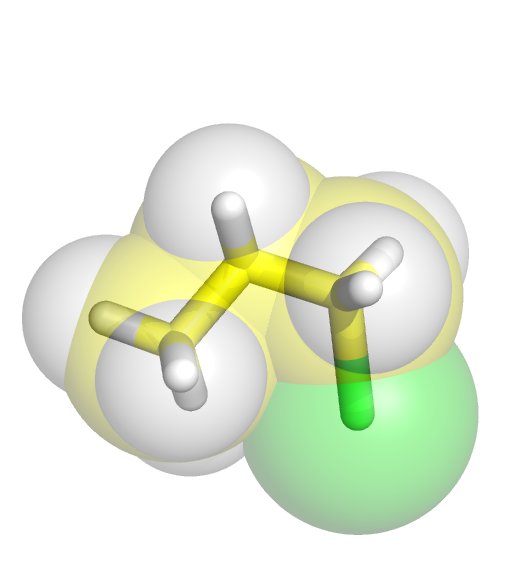
\includegraphics[width=\tmpa]{fig/m003-000} &
%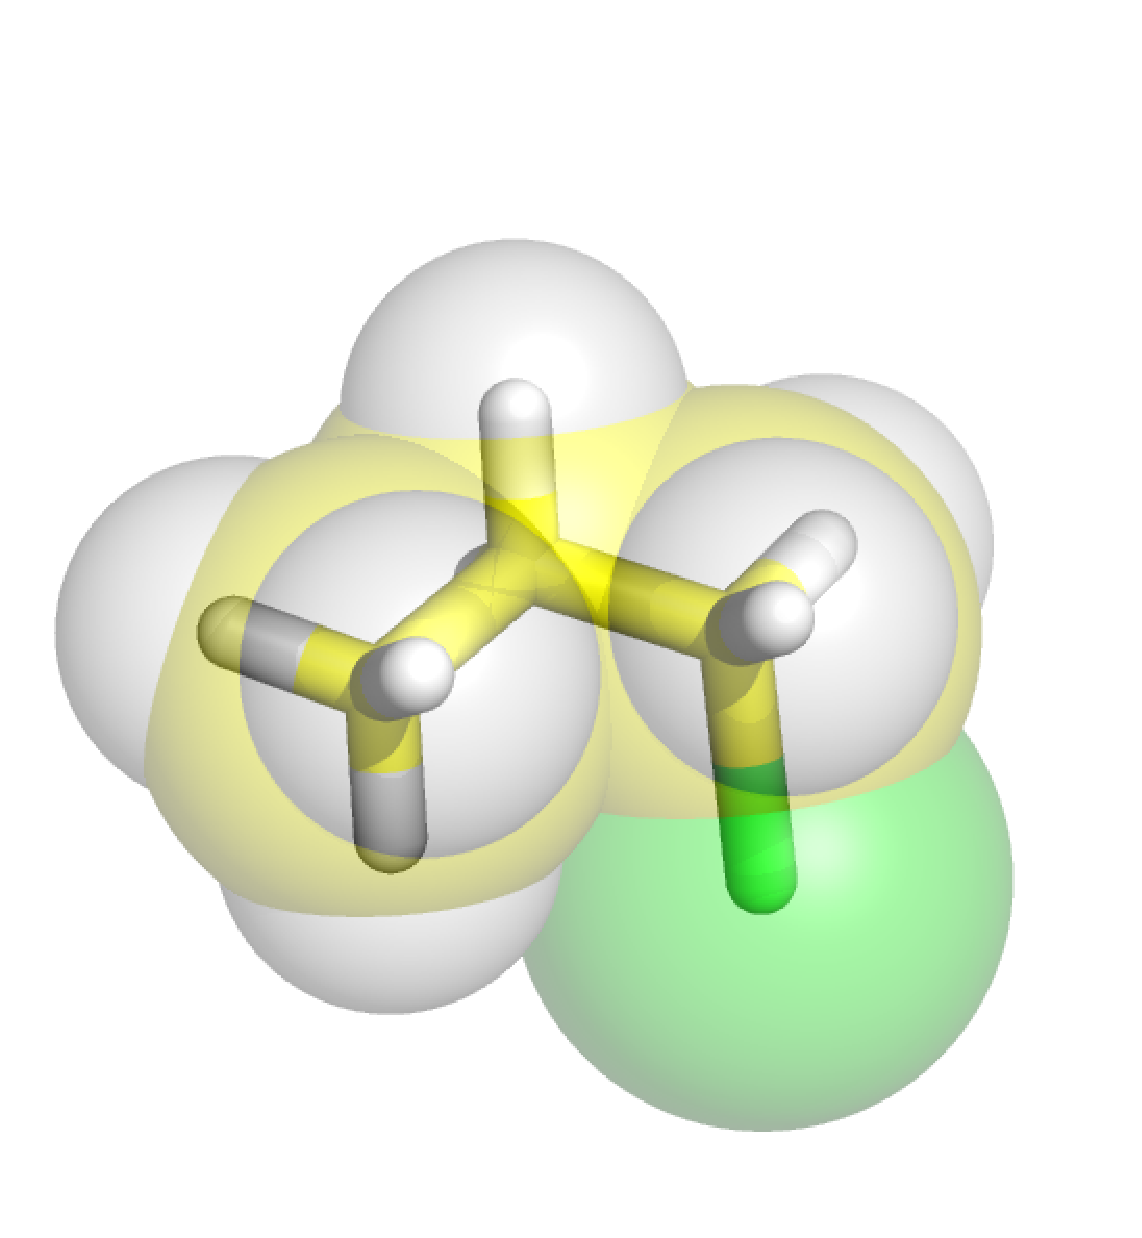
\includegraphics[width=\tmpa]{fig/m003-001} &
%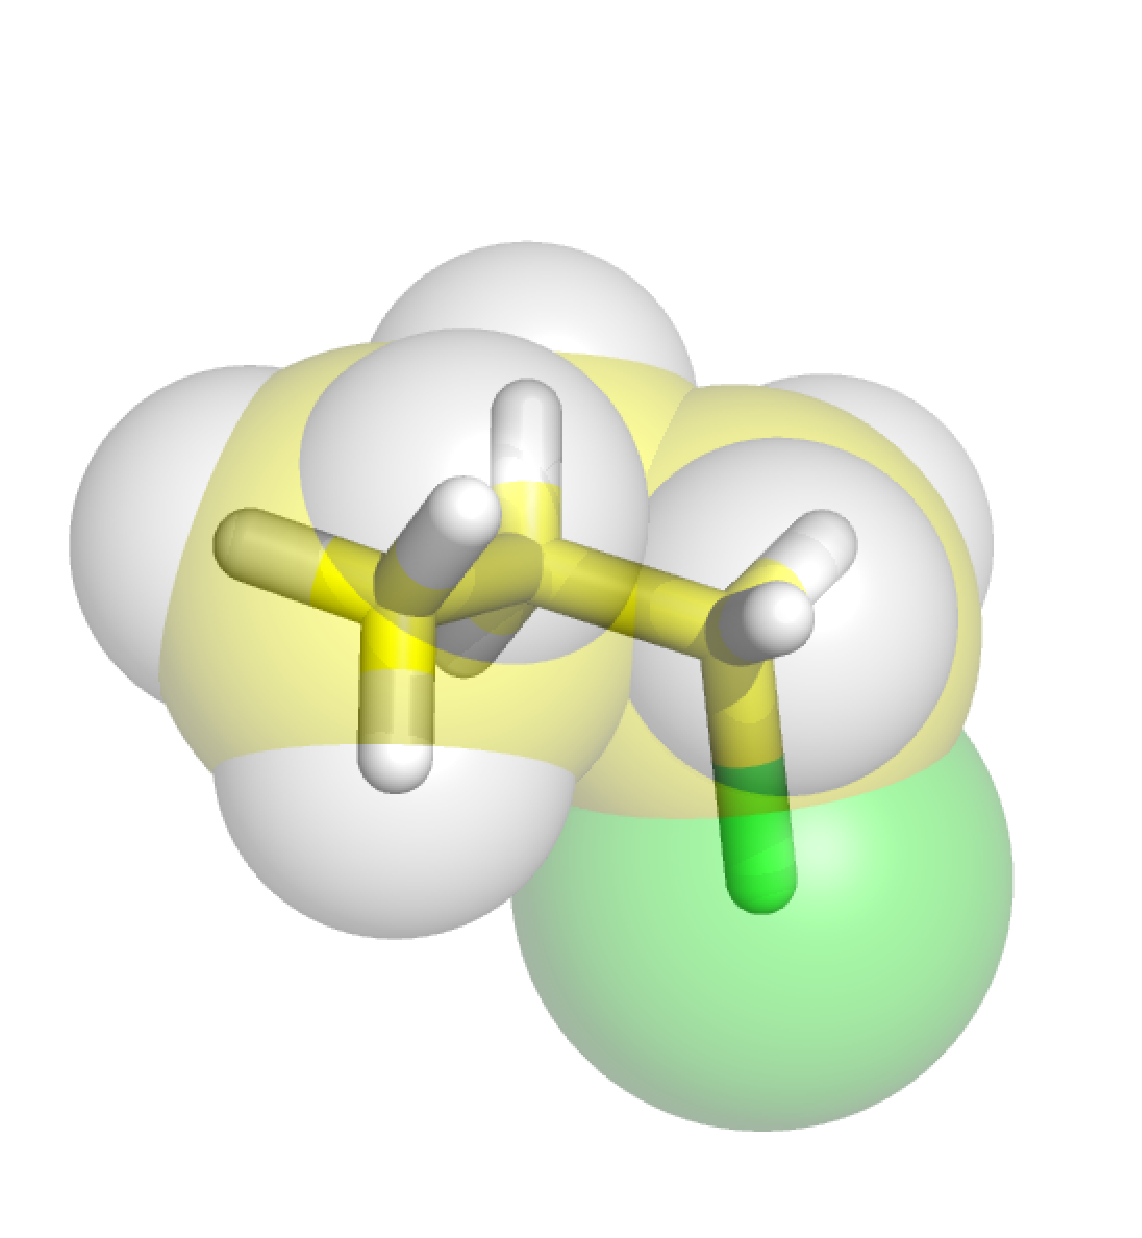
\includegraphics[width=\tmpa]{fig/m003-002} & 
%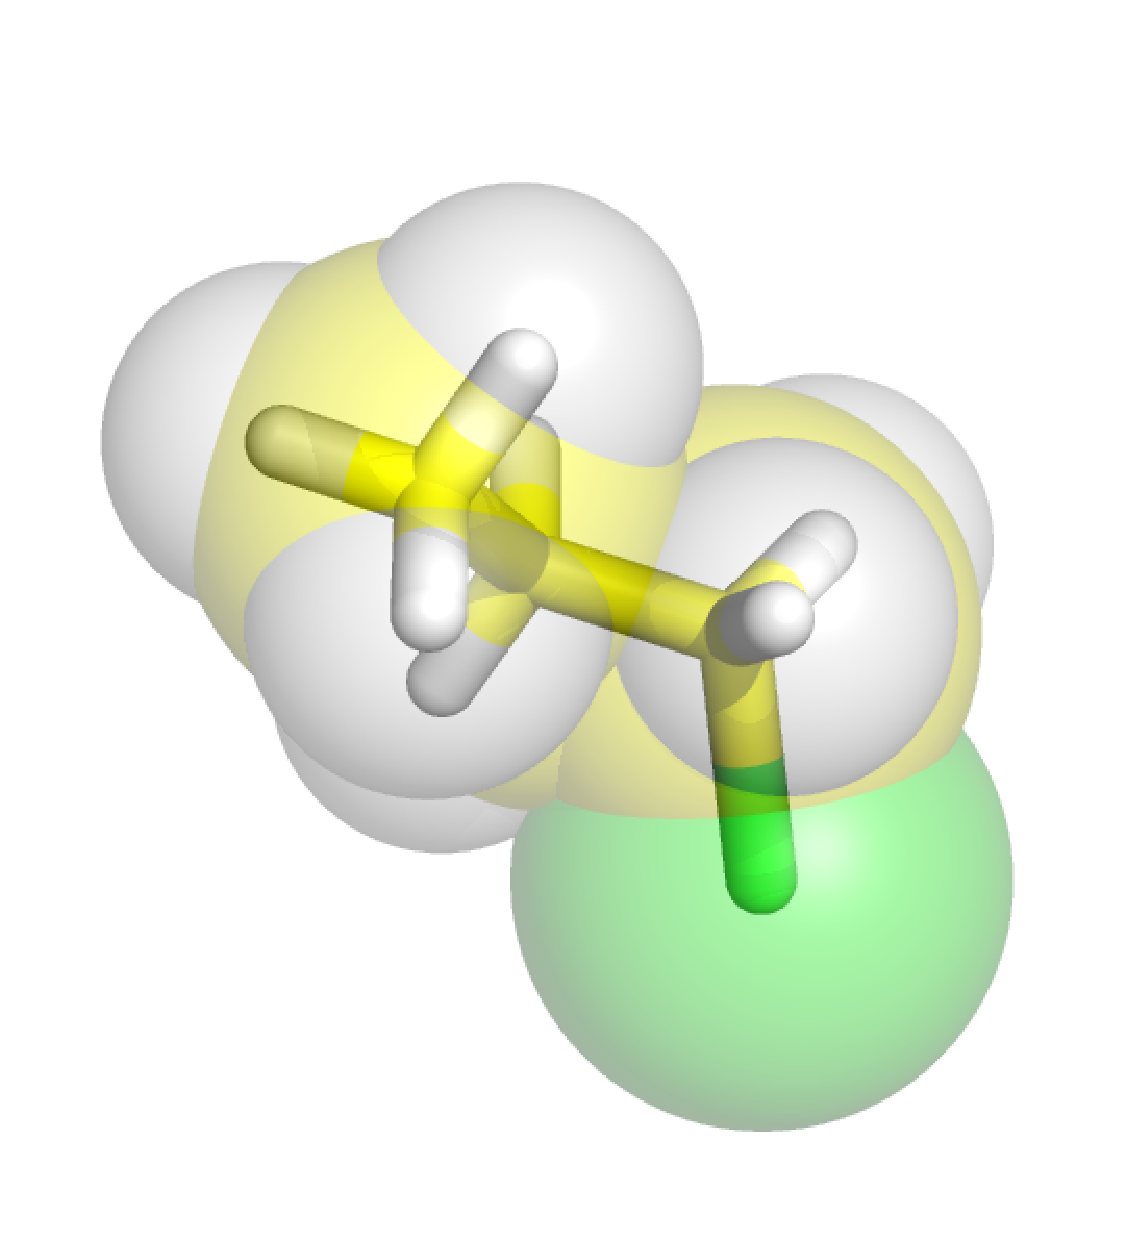
\includegraphics[width=\tmpa]{fig/m003-003} & 
%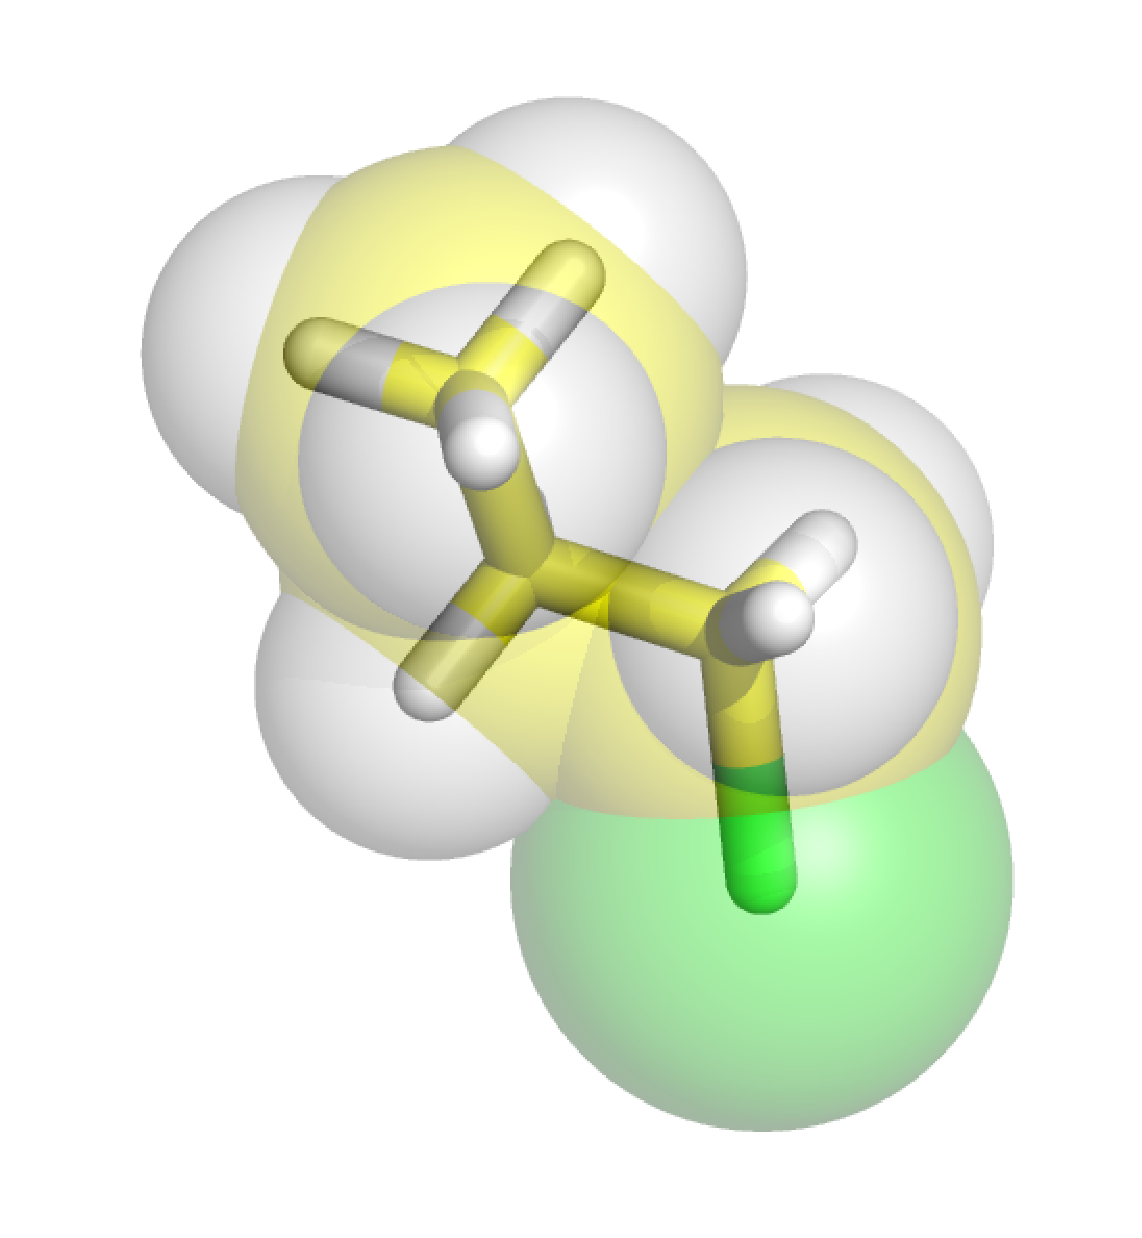
\includegraphics[width=\tmpa]{fig/m003-004} & 
%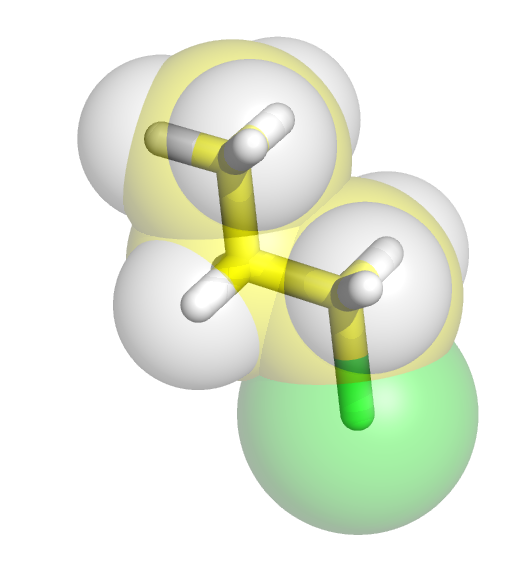
\includegraphics[width=\tmpa]{fig/m003-005} \\
%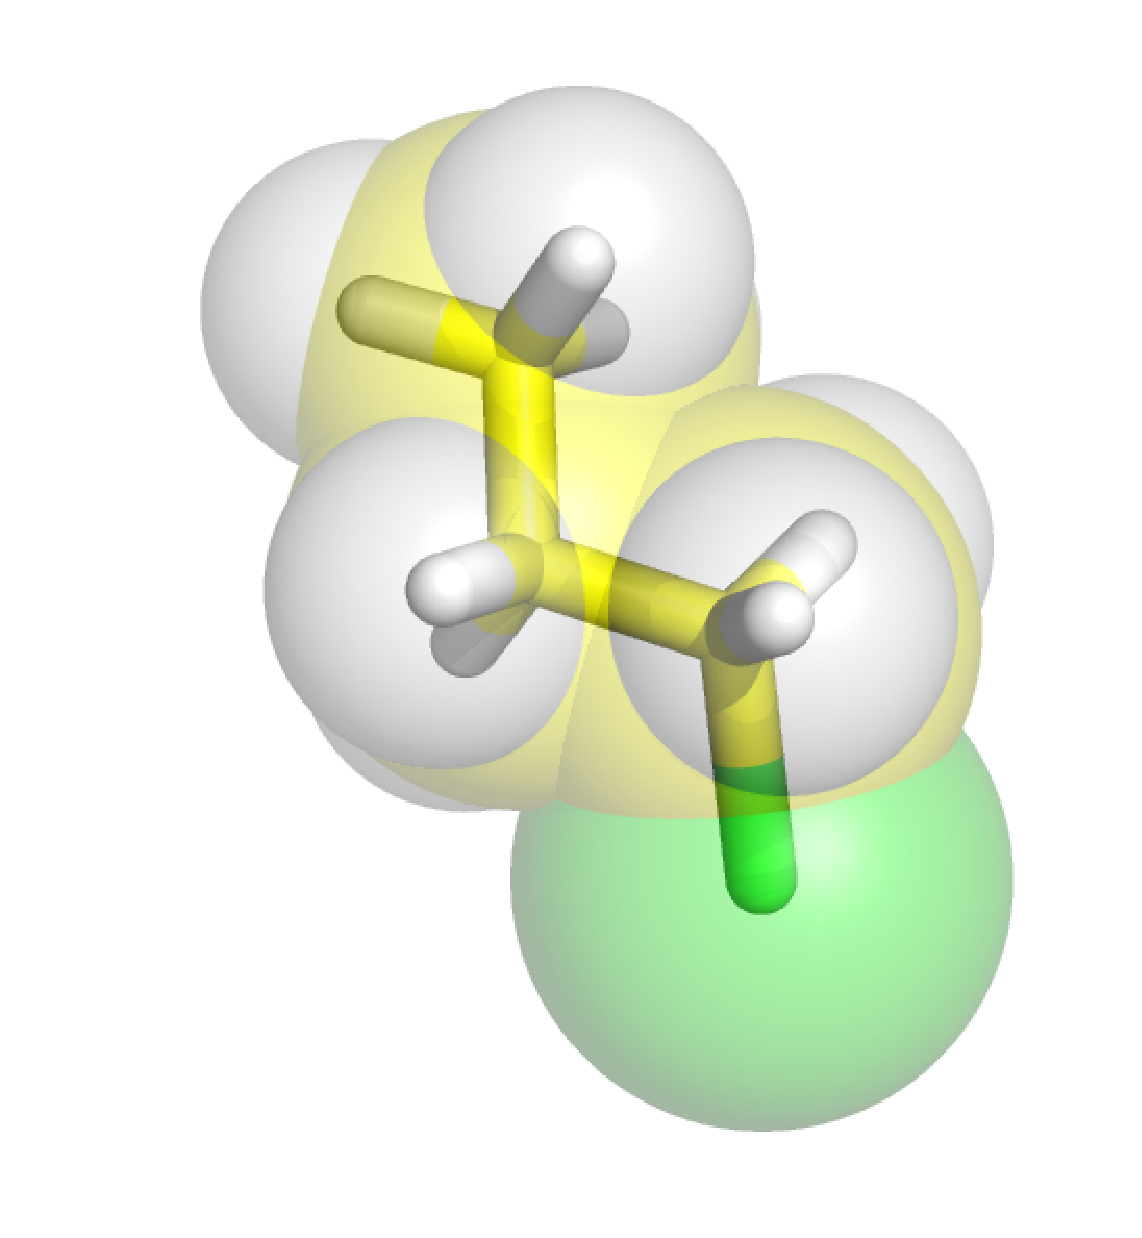
\includegraphics[width=\tmpa]{fig/m003-006} &
%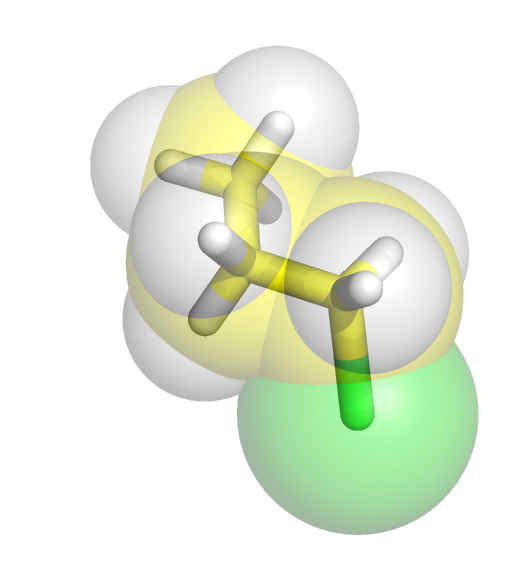
\includegraphics[width=\tmpa]{fig/m003-007} &
%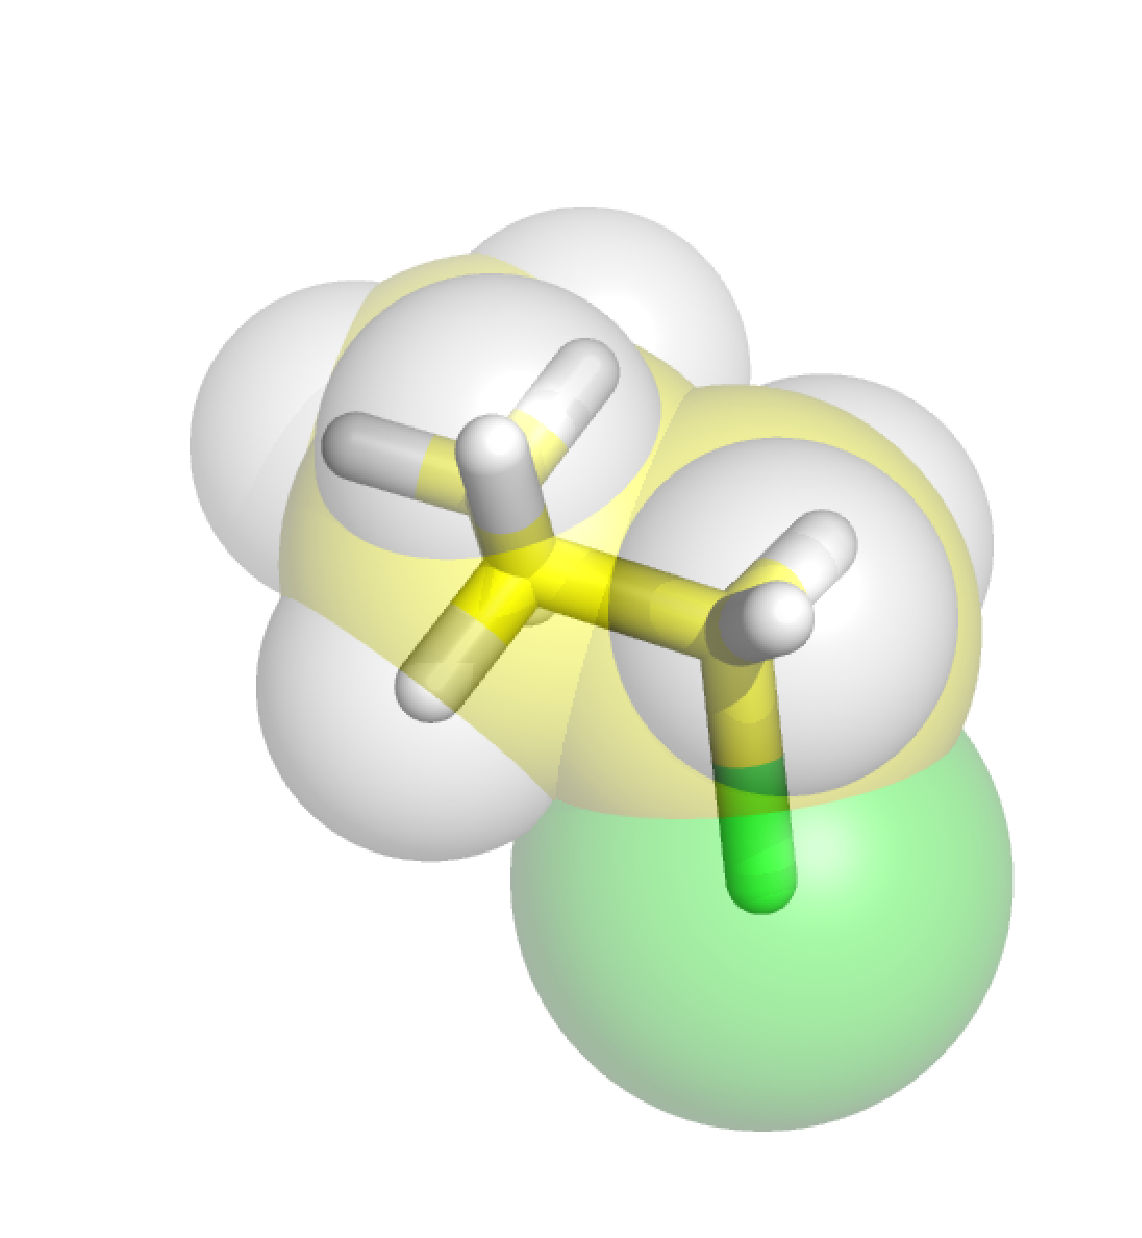
\includegraphics[width=\tmpa]{fig/m003-008} & 
%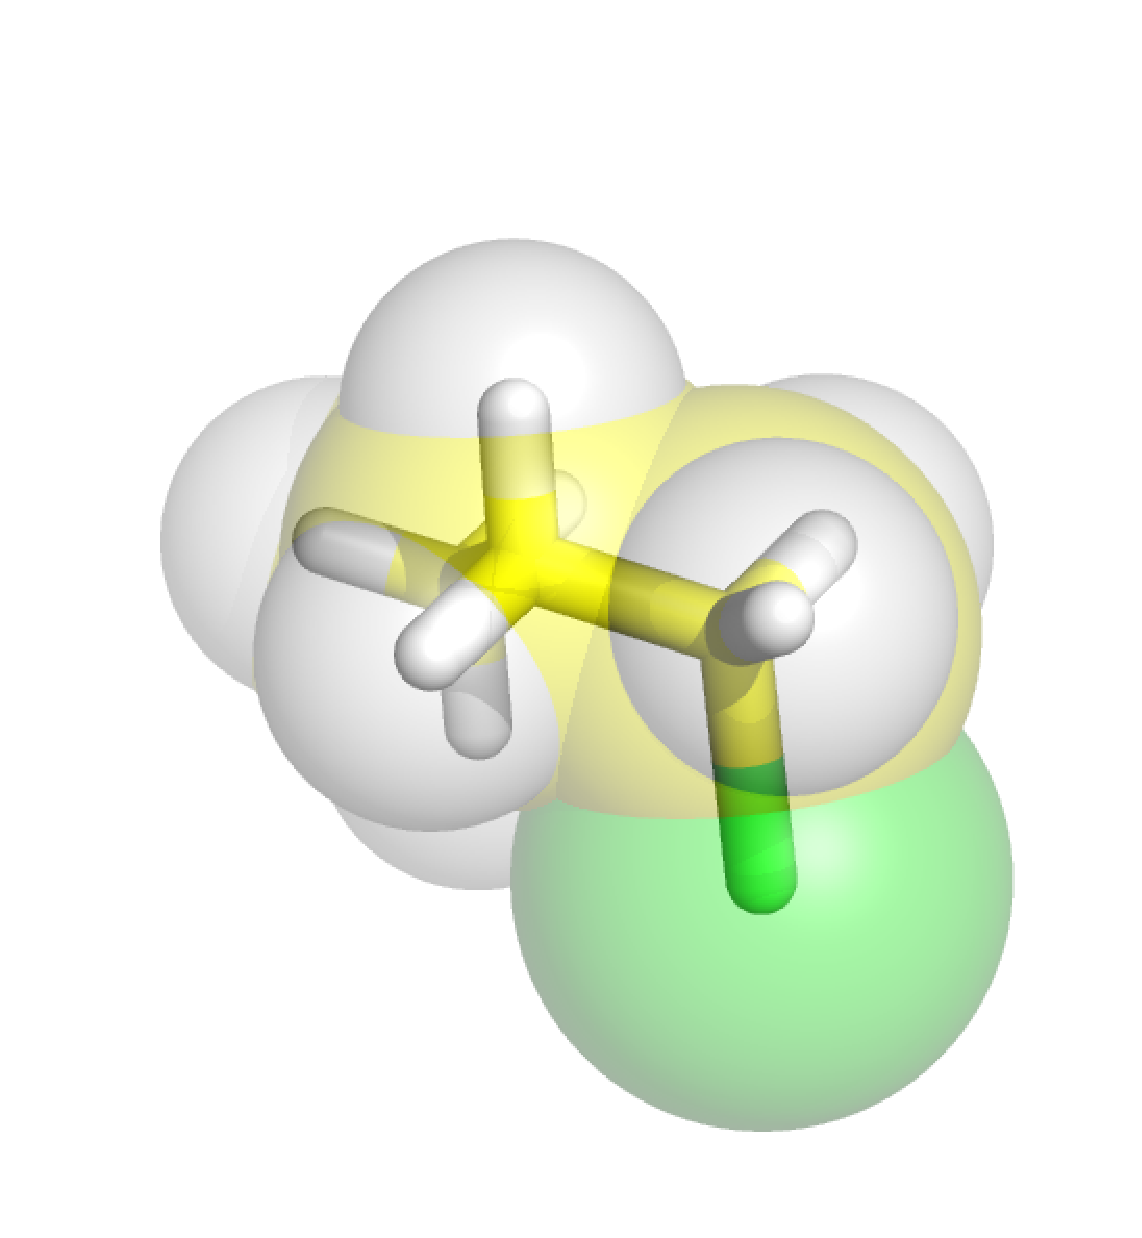
\includegraphics[width=\tmpa]{fig/m003-009} & 
%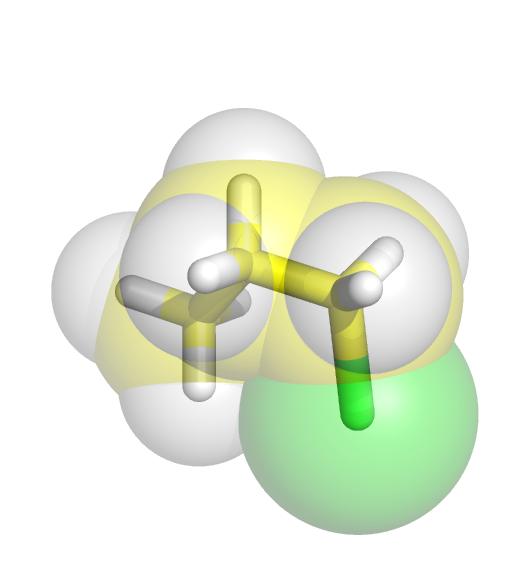
\includegraphics[width=\tmpa]{fig/m003-010} & 
%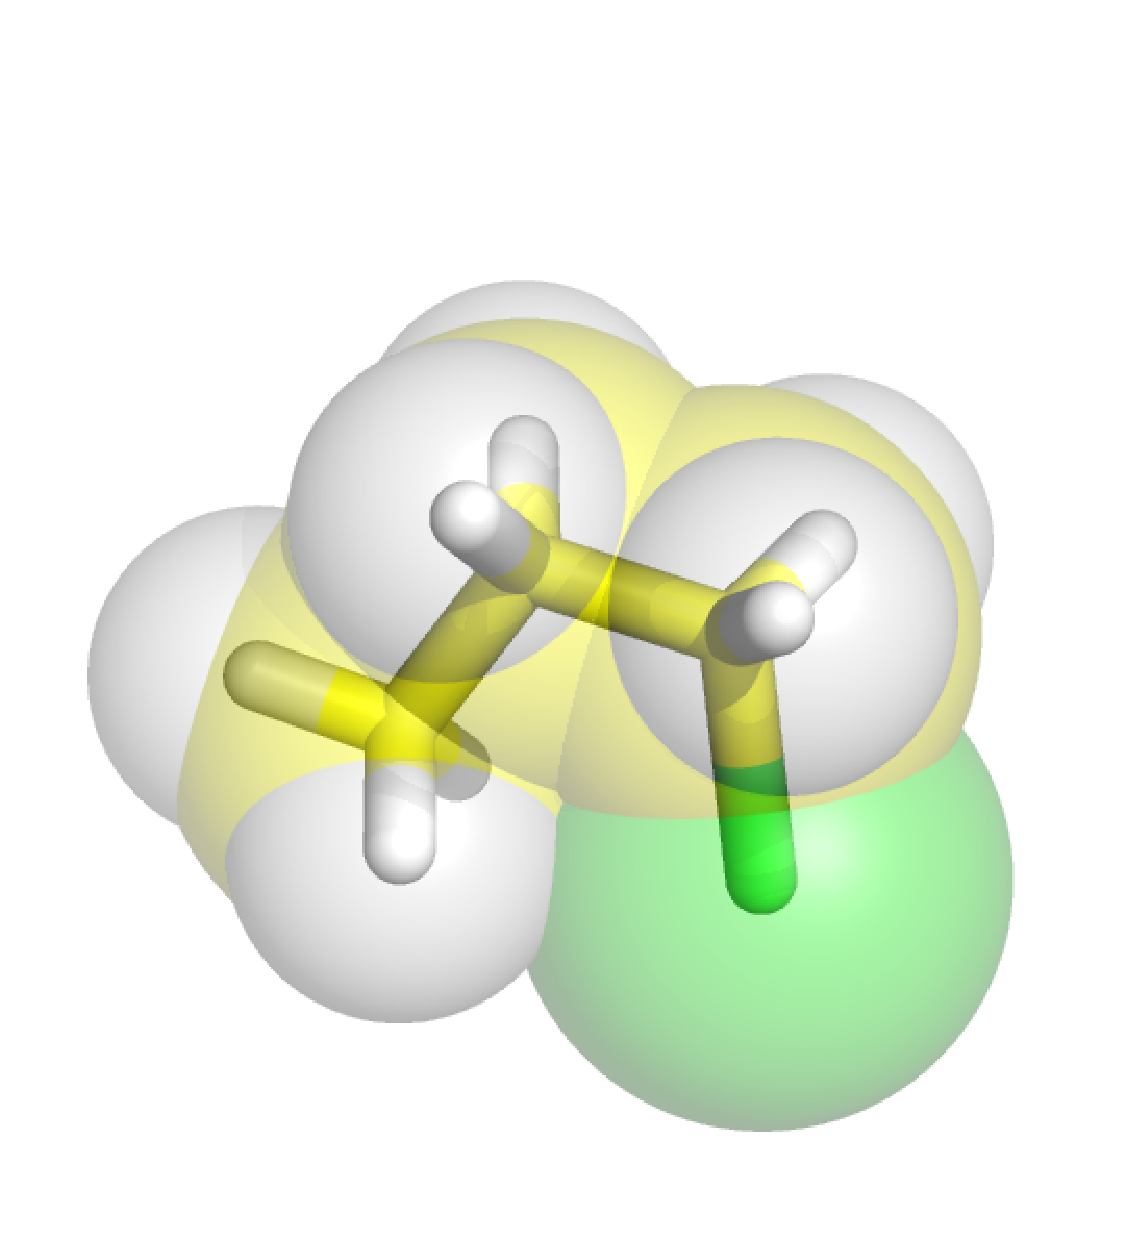
\includegraphics[width=\tmpa]{fig/m003-011} \\
%\end{tabular}
%\caption{todo and maybe delete}
%\end{figure}
%



